\documentclass{beamer}

\usepackage[latin1]{inputenc}
\usepackage{graphicx,epstopdf}
\usepackage{verbatim}
\usepackage{hyperref}
\usepackage{wasysym}
\usepackage{color}

\usepackage{listings}

\usetheme{Warsaw}
\setbeamertemplate{footline}{\hspace{2mm}\insertauthor \;\;\; \insertshorttitle \hspace{40mm} \insertframenumber/\inserttotalframenumber}
\setbeamertemplate{navigation symbols}{}

\title[PPS, Proton POG Meeting]{\large Optics 2018, minimum $x_{0}$ measurement}\vspace{10mm}
\subtitle{\tiny }

\author{F. Nemes}

\begin{document}

\begin{frame}
	\titlepage
\end{frame}

\begin{frame}
	\begin{center}
	\Large
	$x$-angle 130~$\mu$rad, $\beta^{*}=0.25$ m\\ {\small (Run 314276, 2018, April)}
	\end{center}
\end{frame}

\begin{frame}\scriptsize
	\begin{block}{The "neck"}
	RP3, left arm, $s=$213 m
             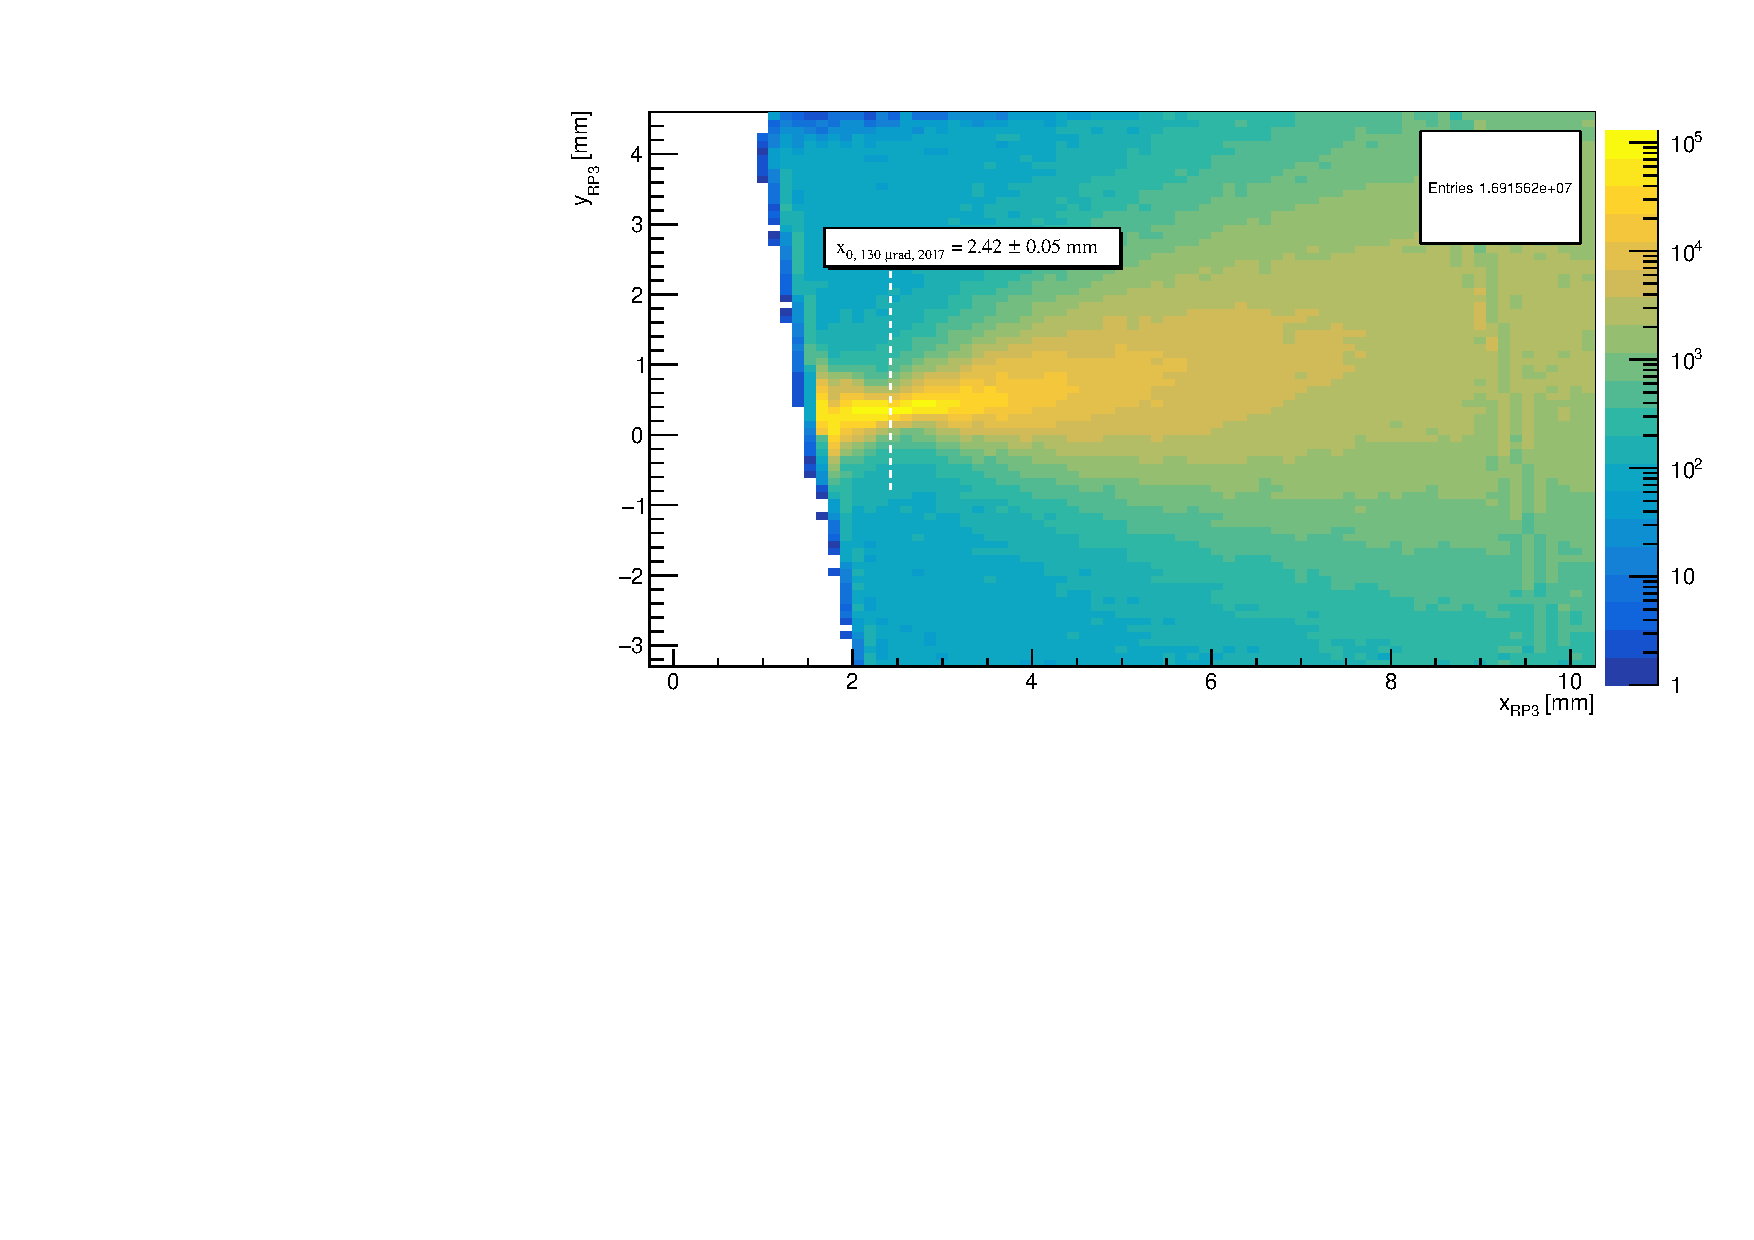
\includegraphics[width=1.0\textwidth]{fig1.pdf}\\
	\end{block}
	
\end{frame}

\begin{frame}\scriptsize
	\begin{block}{Monte Carlo plots: hitmap with and without $\theta_{x}^{*}$}
    		\begin{itemize}
			\item The smearing due to scattering angle
			\item In the data we cannot switch of $L_{x}$ or so
			\item However, one can make a cut on $\theta_{x}$
		\end{itemize}
		\begin{align}
			x = v_{x}\cdot x^{*} + {\color{red} L_{x}\cdot \theta^{*}_{x}}+D_{x}\cdot \xi 	
		\end{align}

             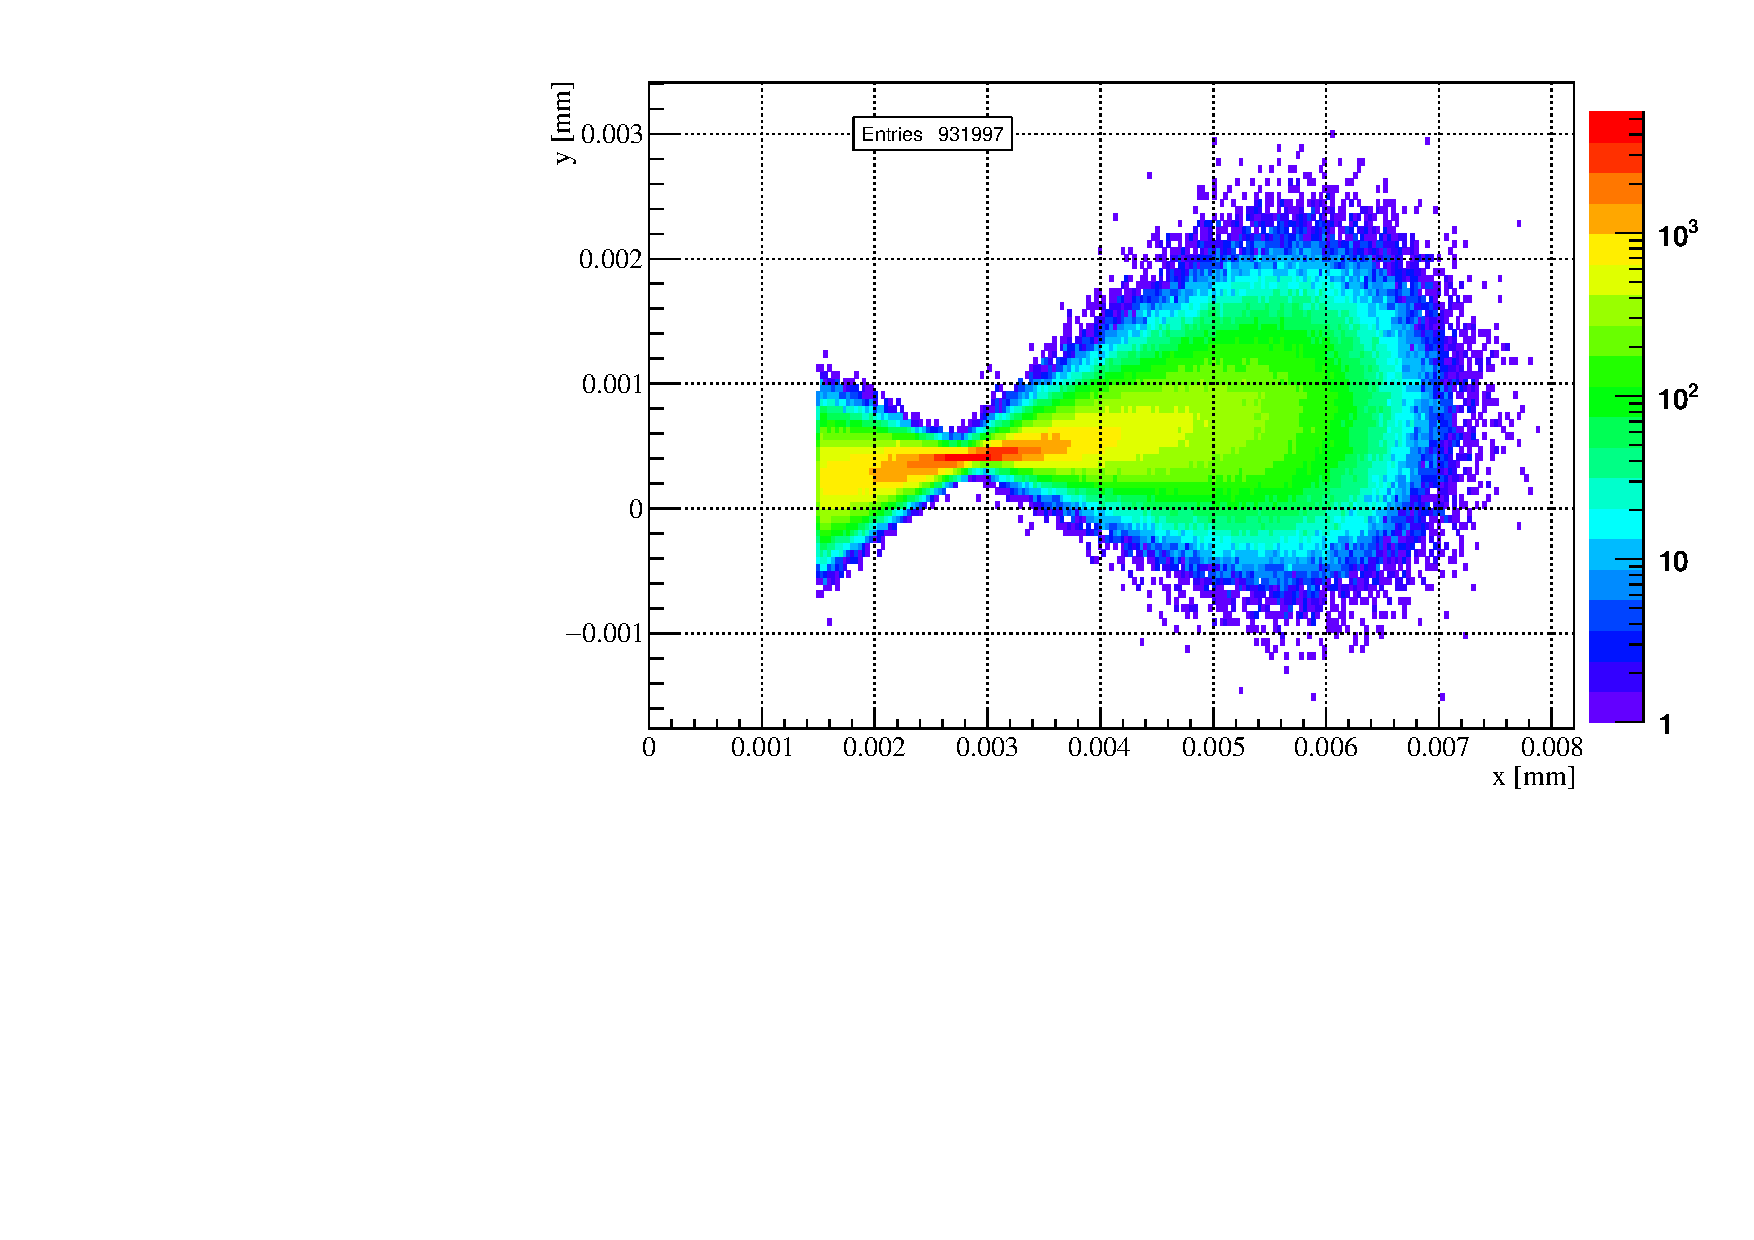
\includegraphics[width=0.48\textwidth]{x_y_hitmap_near.pdf}
             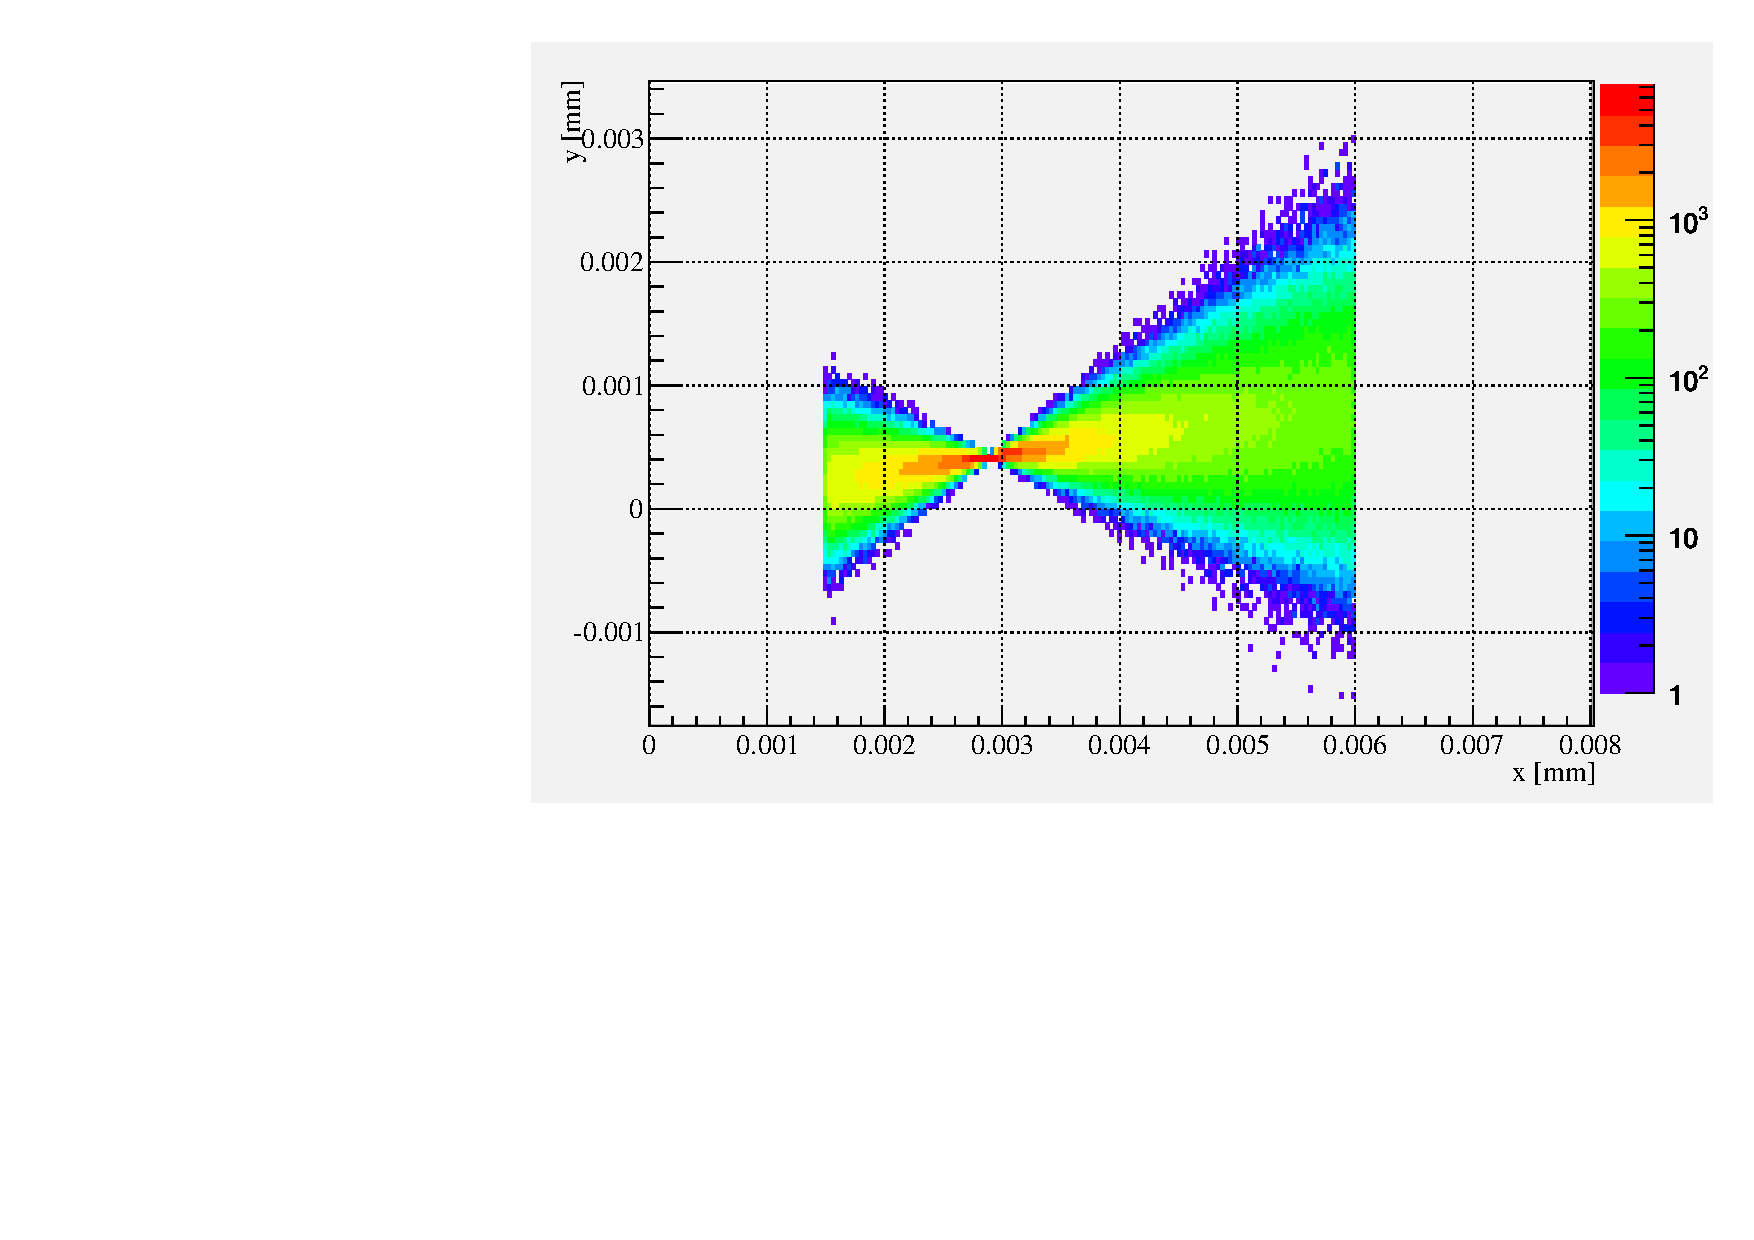
\includegraphics[width=0.48\textwidth]{coll.pdf}
	\end{block}
	
\end{frame}

\begin{frame}\scriptsize
	\begin{block}{The $x$-coordinate difference between RP23 and RP3}
    		\begin{itemize}
			\item Red line shows the cut line (mean)
			\item The $\sigma$ of the cut is 0.0125~mm
		\end{itemize}
             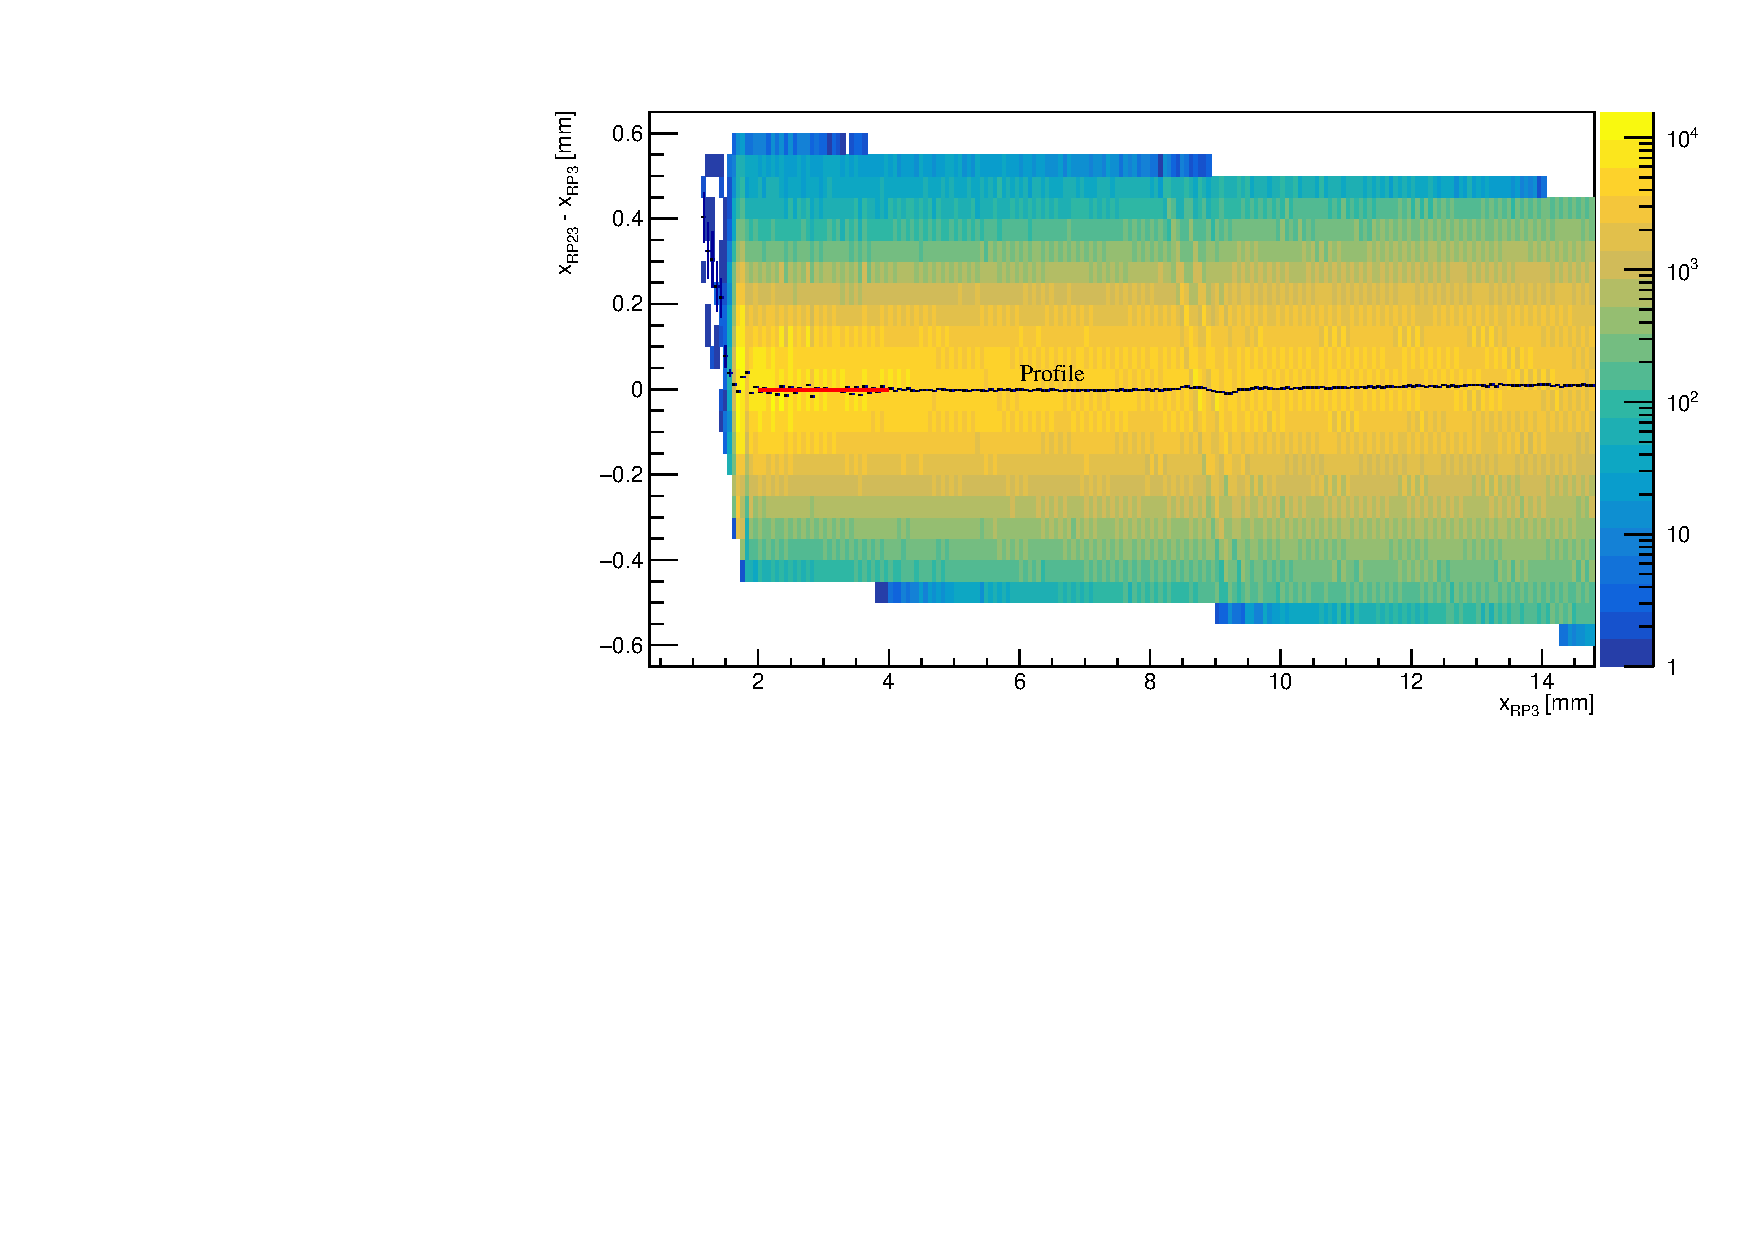
\includegraphics[width=1.0\textwidth]{dxrp23rp3.pdf}\\
	\end{block}
	
\end{frame}

\begin{frame}\scriptsize
	\begin{block}{The x-y hitmap after the dx cut}
    		\begin{itemize}
			\item The angular smearing is close to 0
			\item Note: for these events $\xi_{\rm singleRP}=\xi_{\rm multiRP}$
		\end{itemize}
             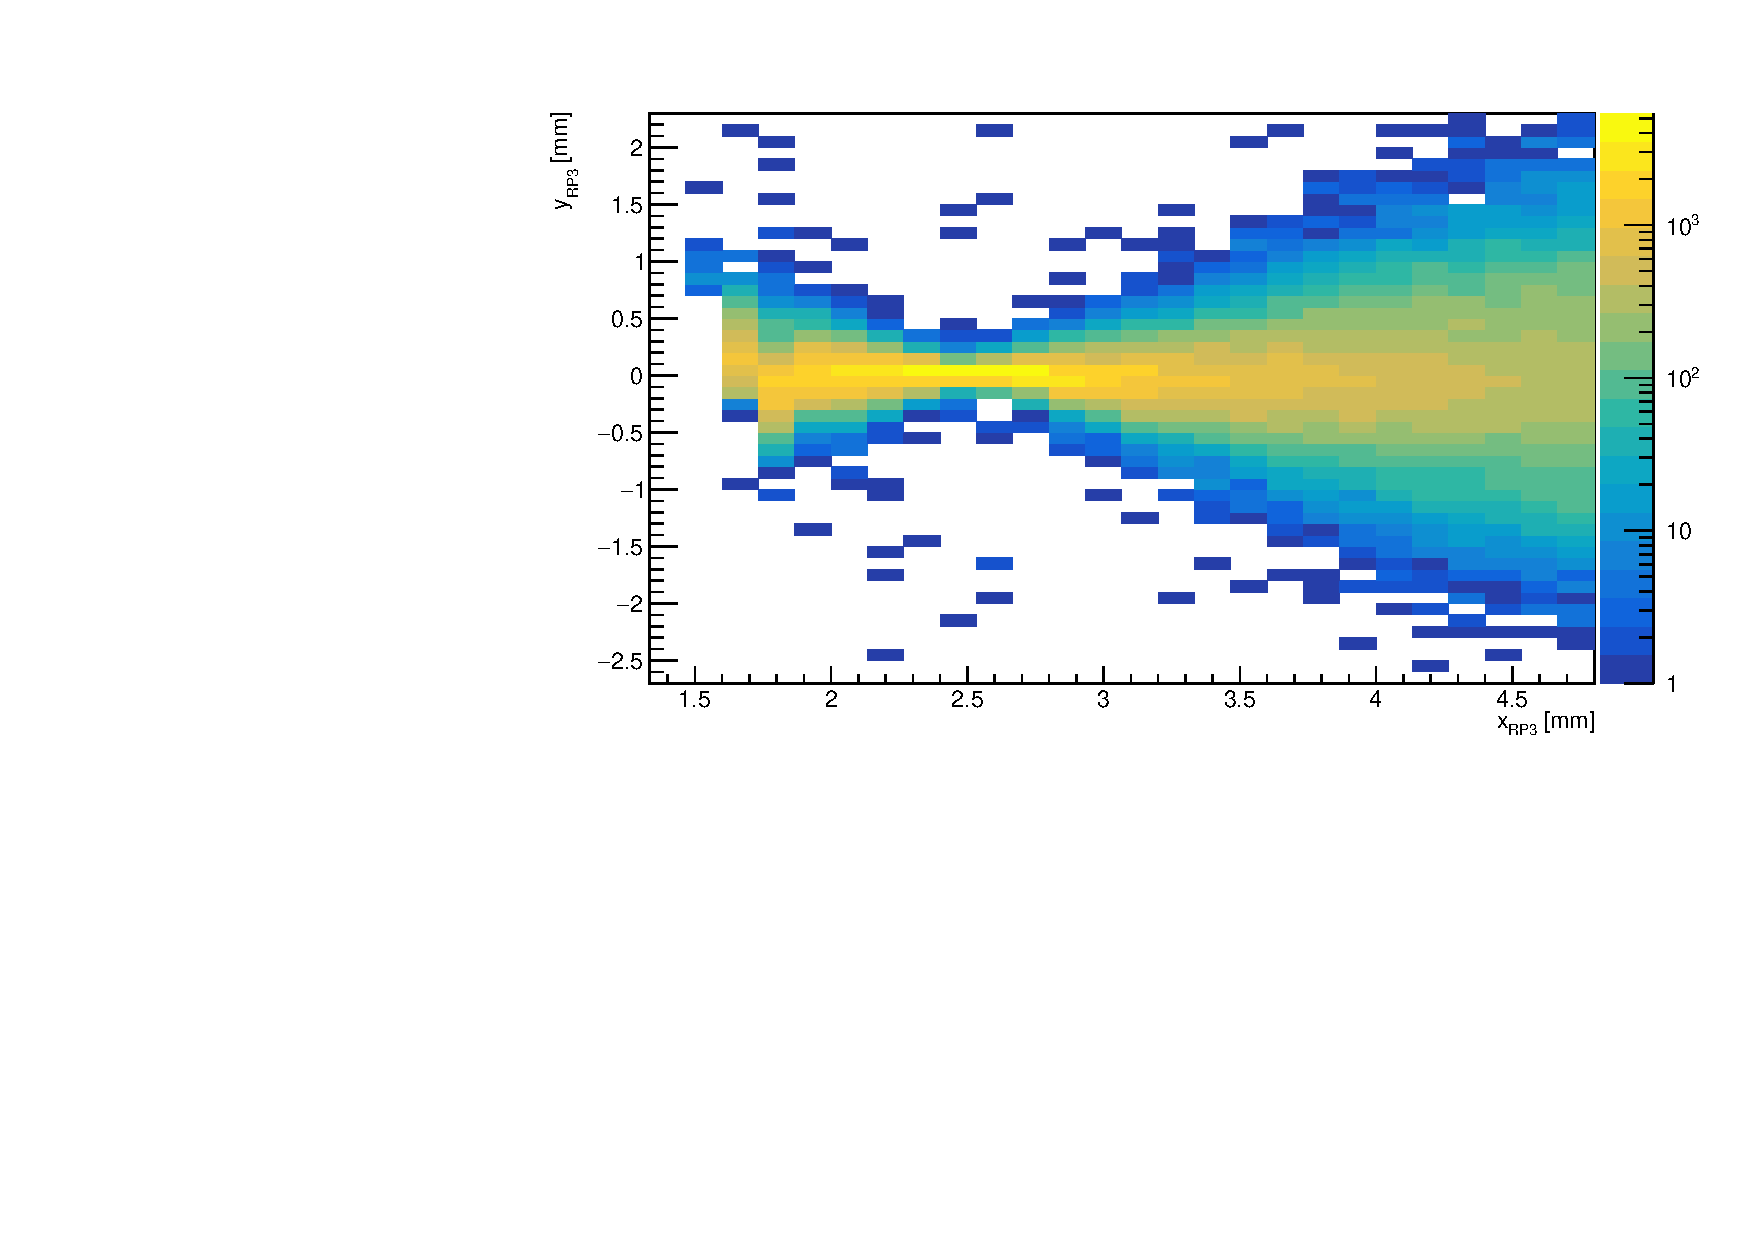
\includegraphics[width=1.0\textwidth]{RP3_after_cut.pdf}\\
	\end{block}
	
\end{frame}

\begin{frame}\scriptsize
	\begin{block}{The RMS of the $y$-coordinate}
    		\begin{itemize}
			\item The minimum shows the quick $L_{y}$ cross-over 0
		\end{itemize}
             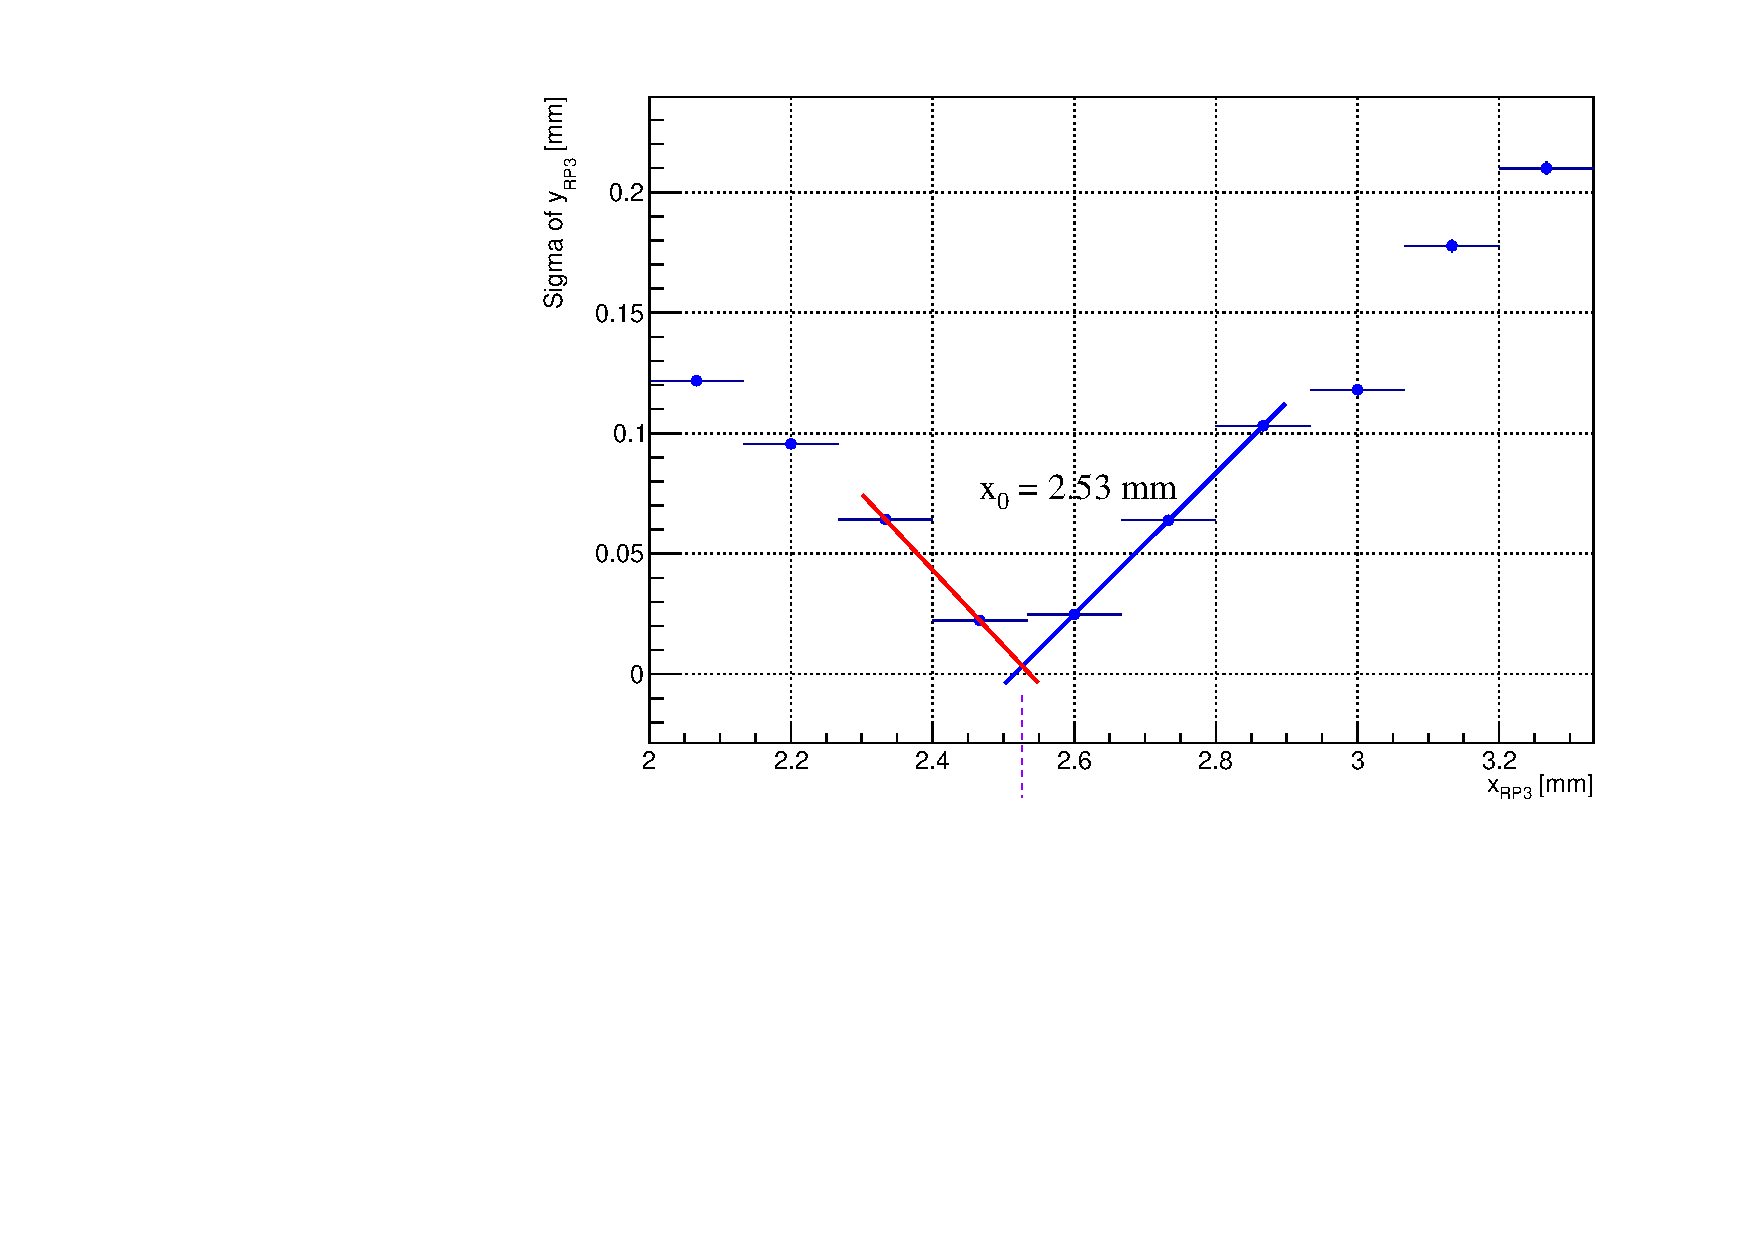
\includegraphics[width=1.0\textwidth]{x0130muradrp3.pdf}\\
	\end{block}
	
\end{frame}


\begin{frame}
	\begin{center}
	\Large
	$x$-angle 160~$\mu$rad	\\ {\small (Run 314247, 2018, April)}
	\end{center}
\end{frame}

\begin{frame}\scriptsize
	\begin{block}{The RP3 x-y hitmap after the dx cut}
             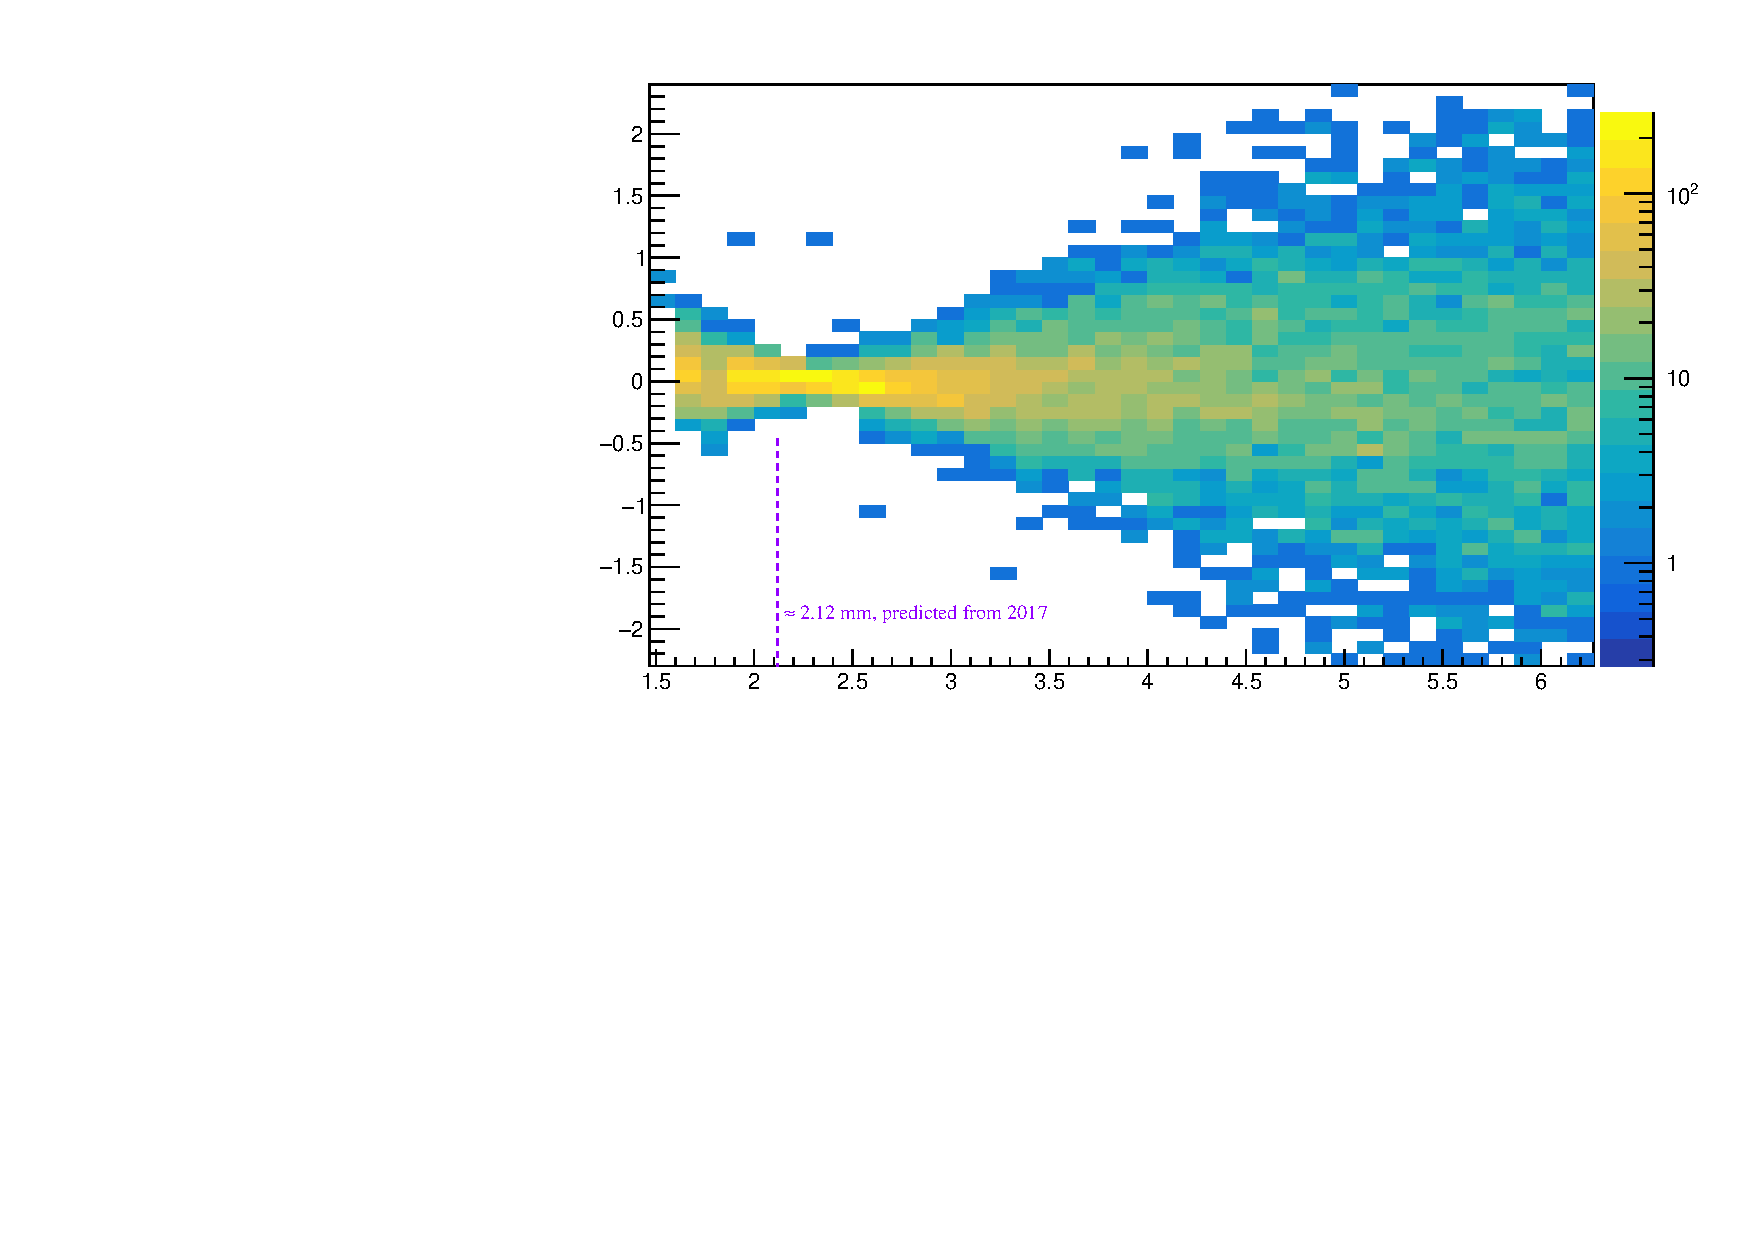
\includegraphics[width=1.0\textwidth]{160murad_neck.pdf}
	\end{block}
	
\end{frame}


\begin{frame}\scriptsize
	\begin{block}{The RMS of the $y$-coordinate and $x_{0}$}
    		\begin{itemize}
			\item A bit unexpected (see later with September 130 $\mu$rad data)
			\item Would break dispersion as function of x-angle from 2017
		\end{itemize}
             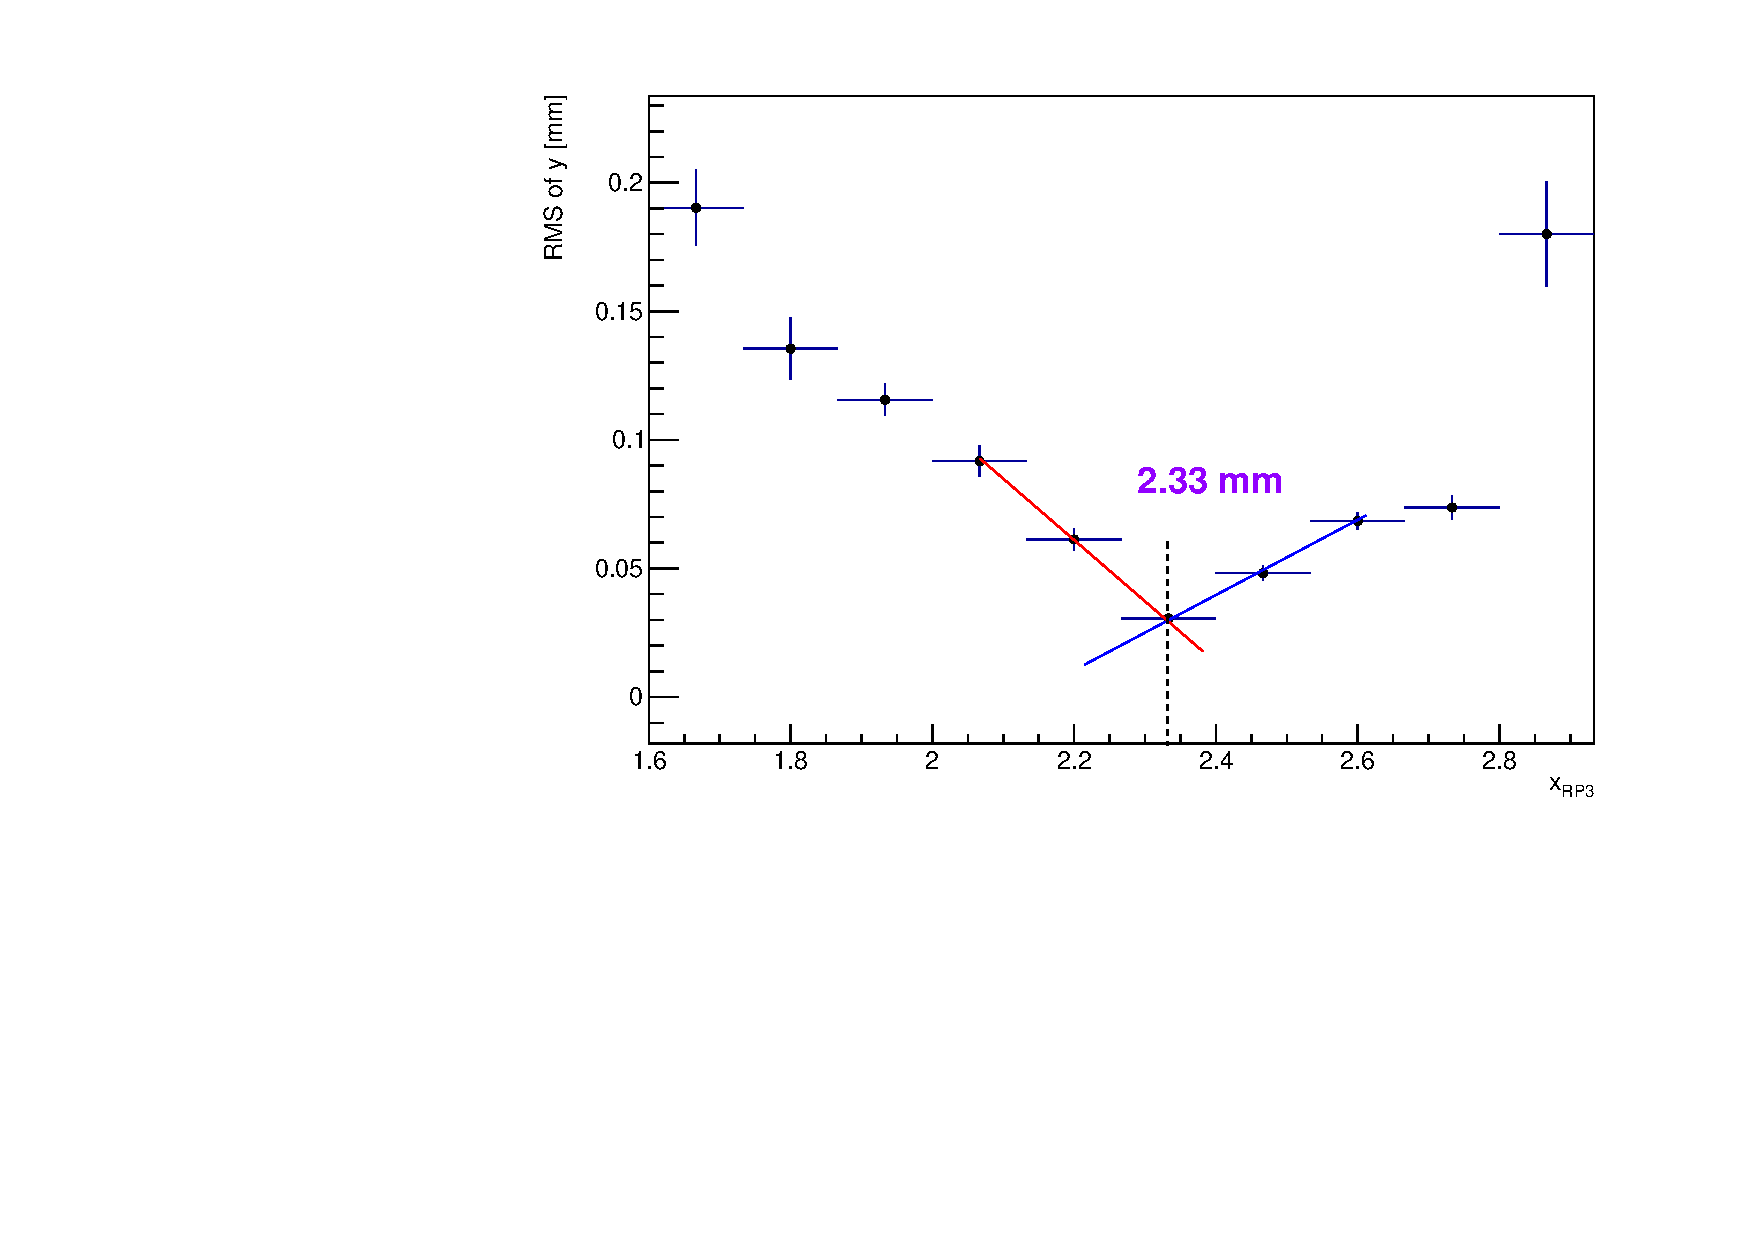
\includegraphics[width=1.0\textwidth]{160muradRMS.pdf}
	\end{block}
	
\end{frame}

\begin{frame}\scriptsize
	\begin{block}{Overlap between RP3, 4 and 5}
             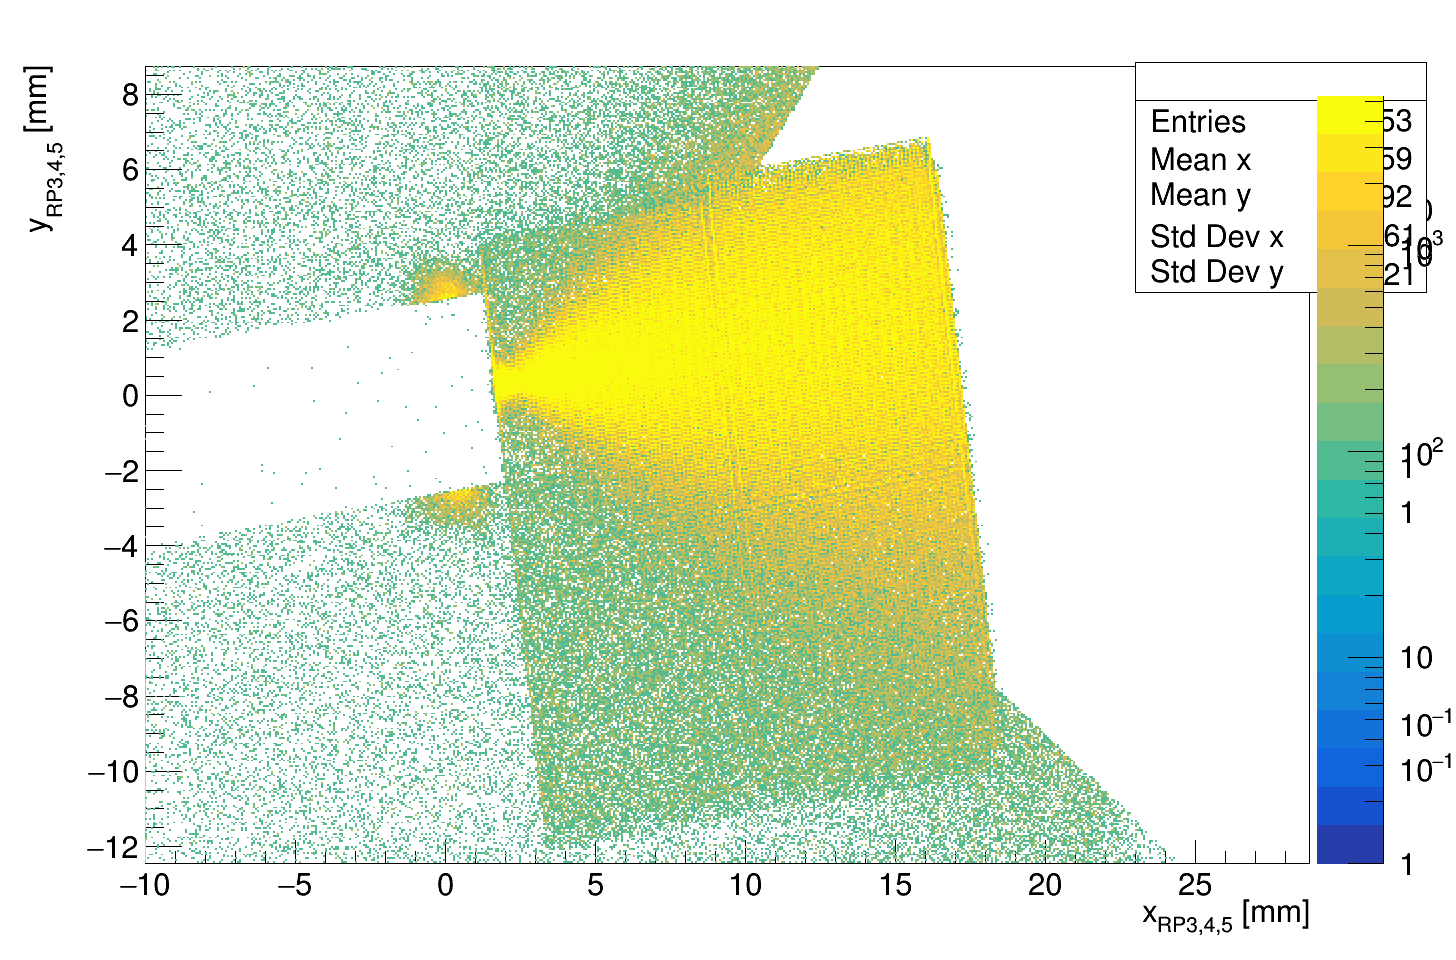
\includegraphics[width=1.0\textwidth]{overlap.png}
	\end{block}
	
\end{frame}

\begin{frame}\scriptsize
	\begin{block}{Horizontal alignment test between RP3, 4 and 5}
             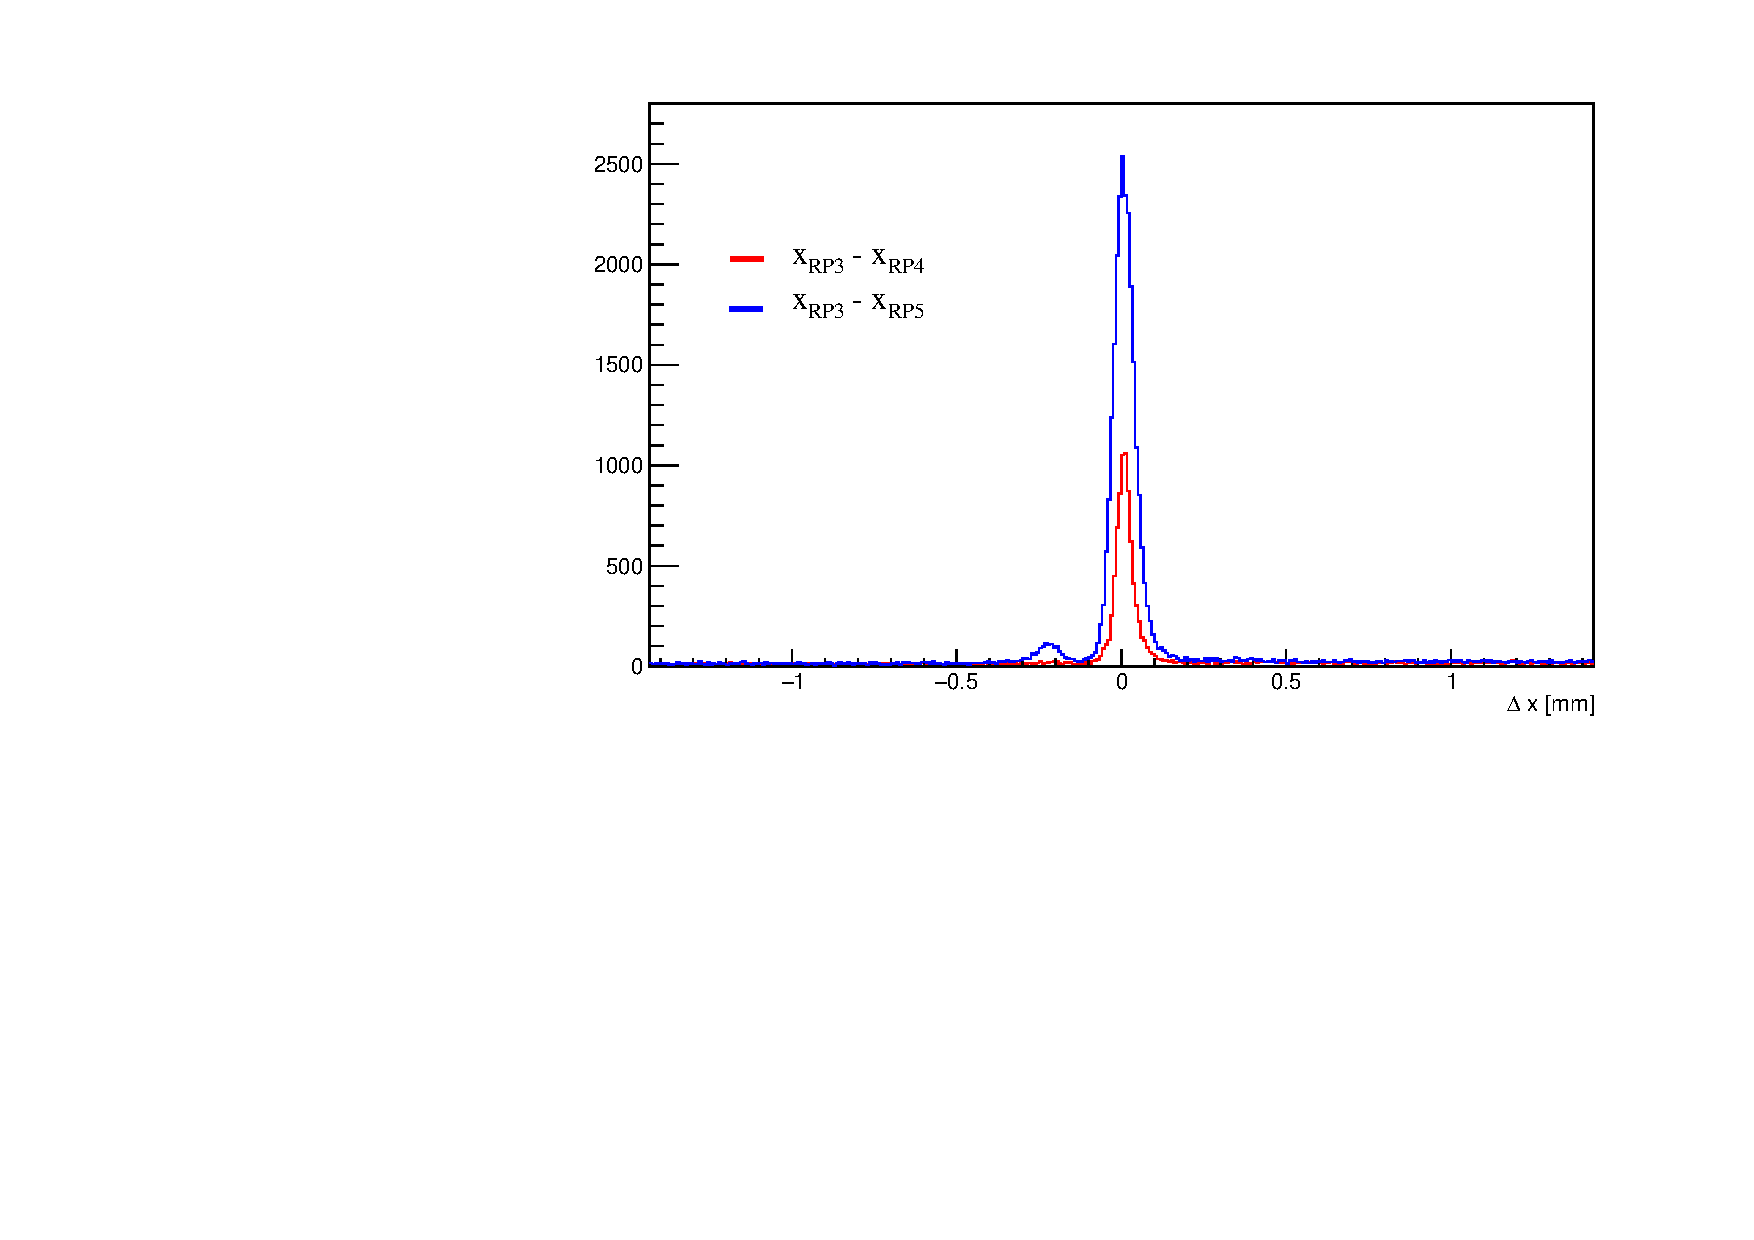
\includegraphics[width=1.0\textwidth]{x_alignment_160_murad.pdf}
	\end{block}
	
\end{frame}

\begin{frame}\scriptsize
	\begin{block}{Elastics at 160~$\mu$rad: single arm correlations}
    		\begin{itemize}
			\item RP4 and 24: top verticals
			\item TOTEM methods to identify elastics
			\item Note: focusing
		\end{itemize}
	\begin{center}
             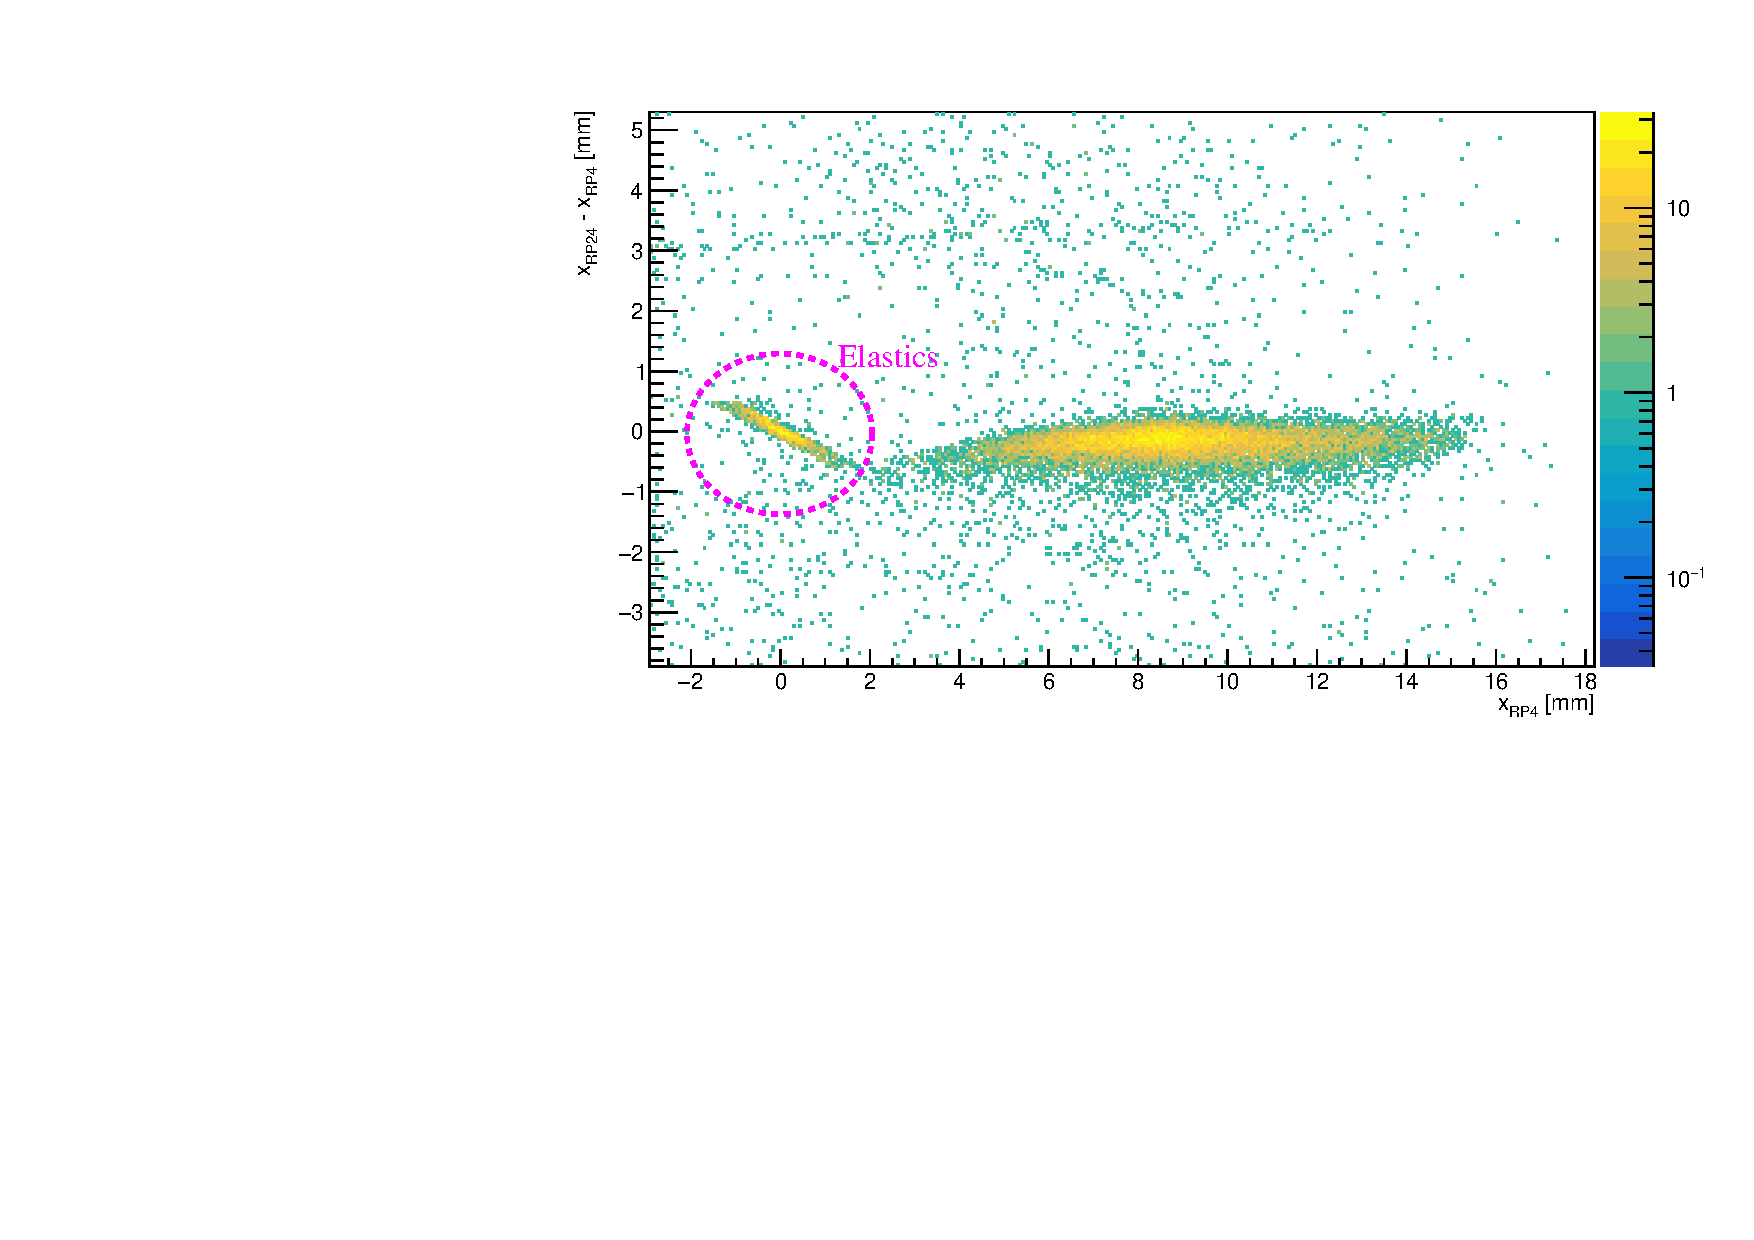
\includegraphics[width=0.48\textwidth]{160_murad_x_elastics.pdf}
             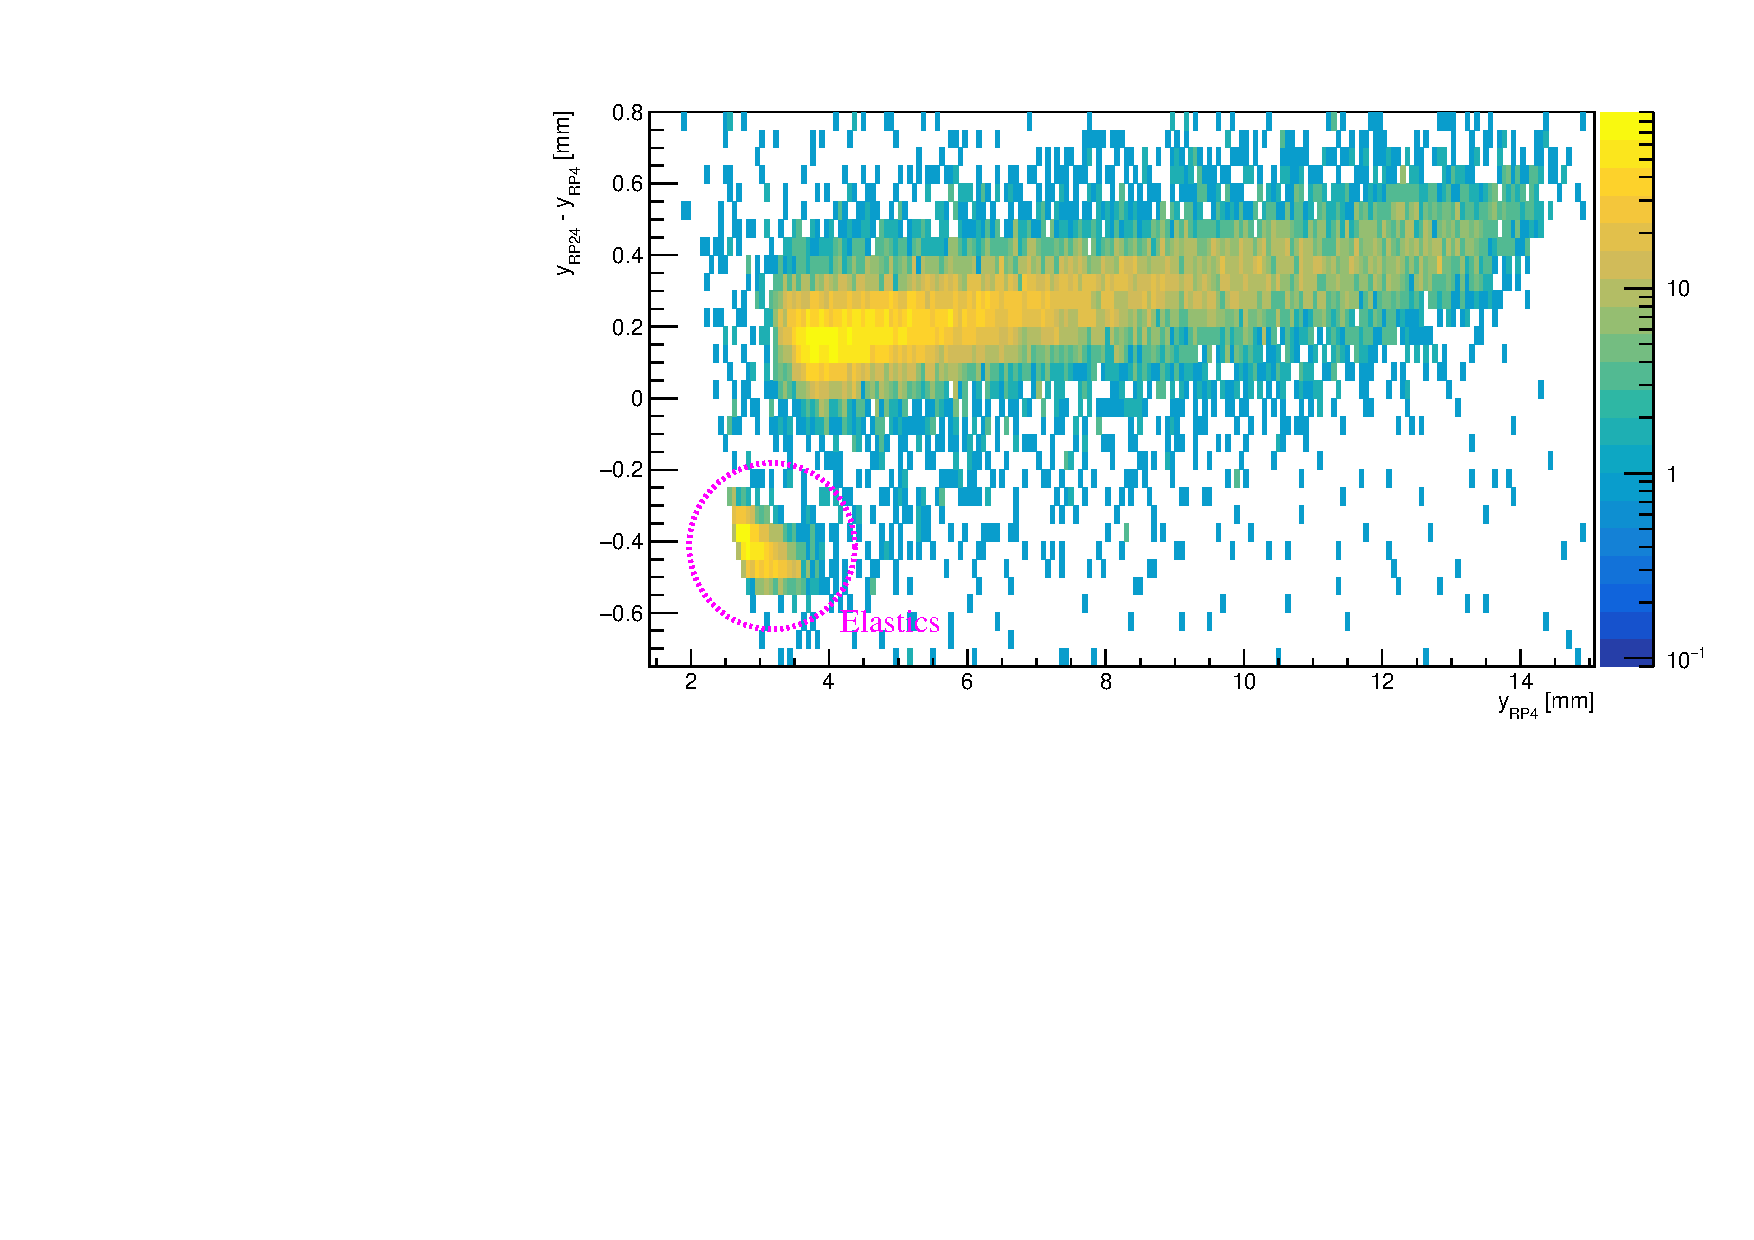
\includegraphics[width=0.48\textwidth]{160_murad_y_elastics.pdf}\\
	\end{center}
	\end{block}
	
\end{frame}


\begin{frame}\scriptsize
	\begin{block}{Elastics at 160~$\mu$rad: test of absolute horizontal alignment}
    		\begin{itemize}
			\item $x_{0}\approx$ 2.33 - 0.23 = 2.1 mm
		\end{itemize}
	\begin{center}
            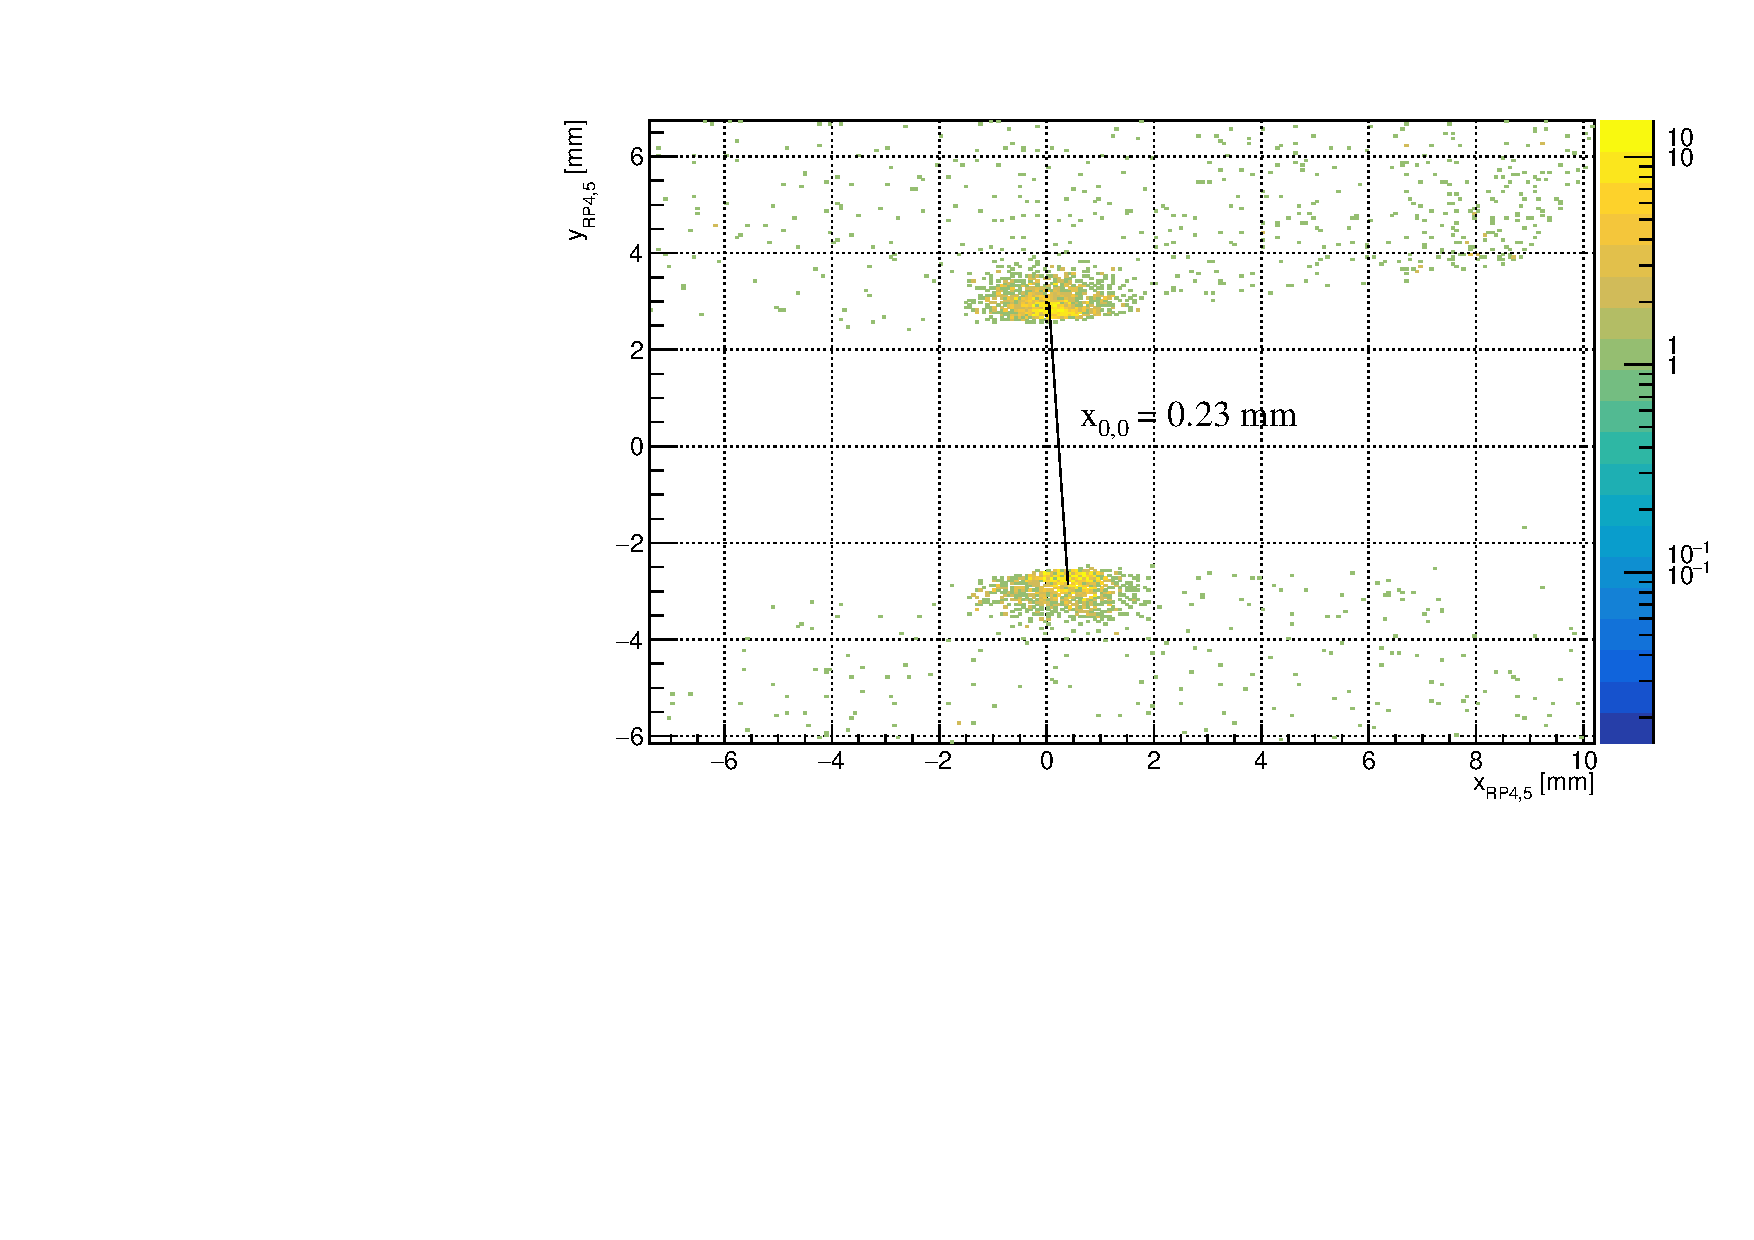
\includegraphics[width=0.8\textwidth]{beam_spot.pdf}
	\end{center}
	\end{block}
	
\end{frame}

\begin{frame}
	\begin{center}
	\Large
	Remaining alignment tests for $x$-angle 130~$\mu$rad
	\\ {\small (2018, April)}
	\end{center}
\end{frame}

\begin{frame}\scriptsize
	\begin{block}{Overlap between RP3, 4 and 5}
             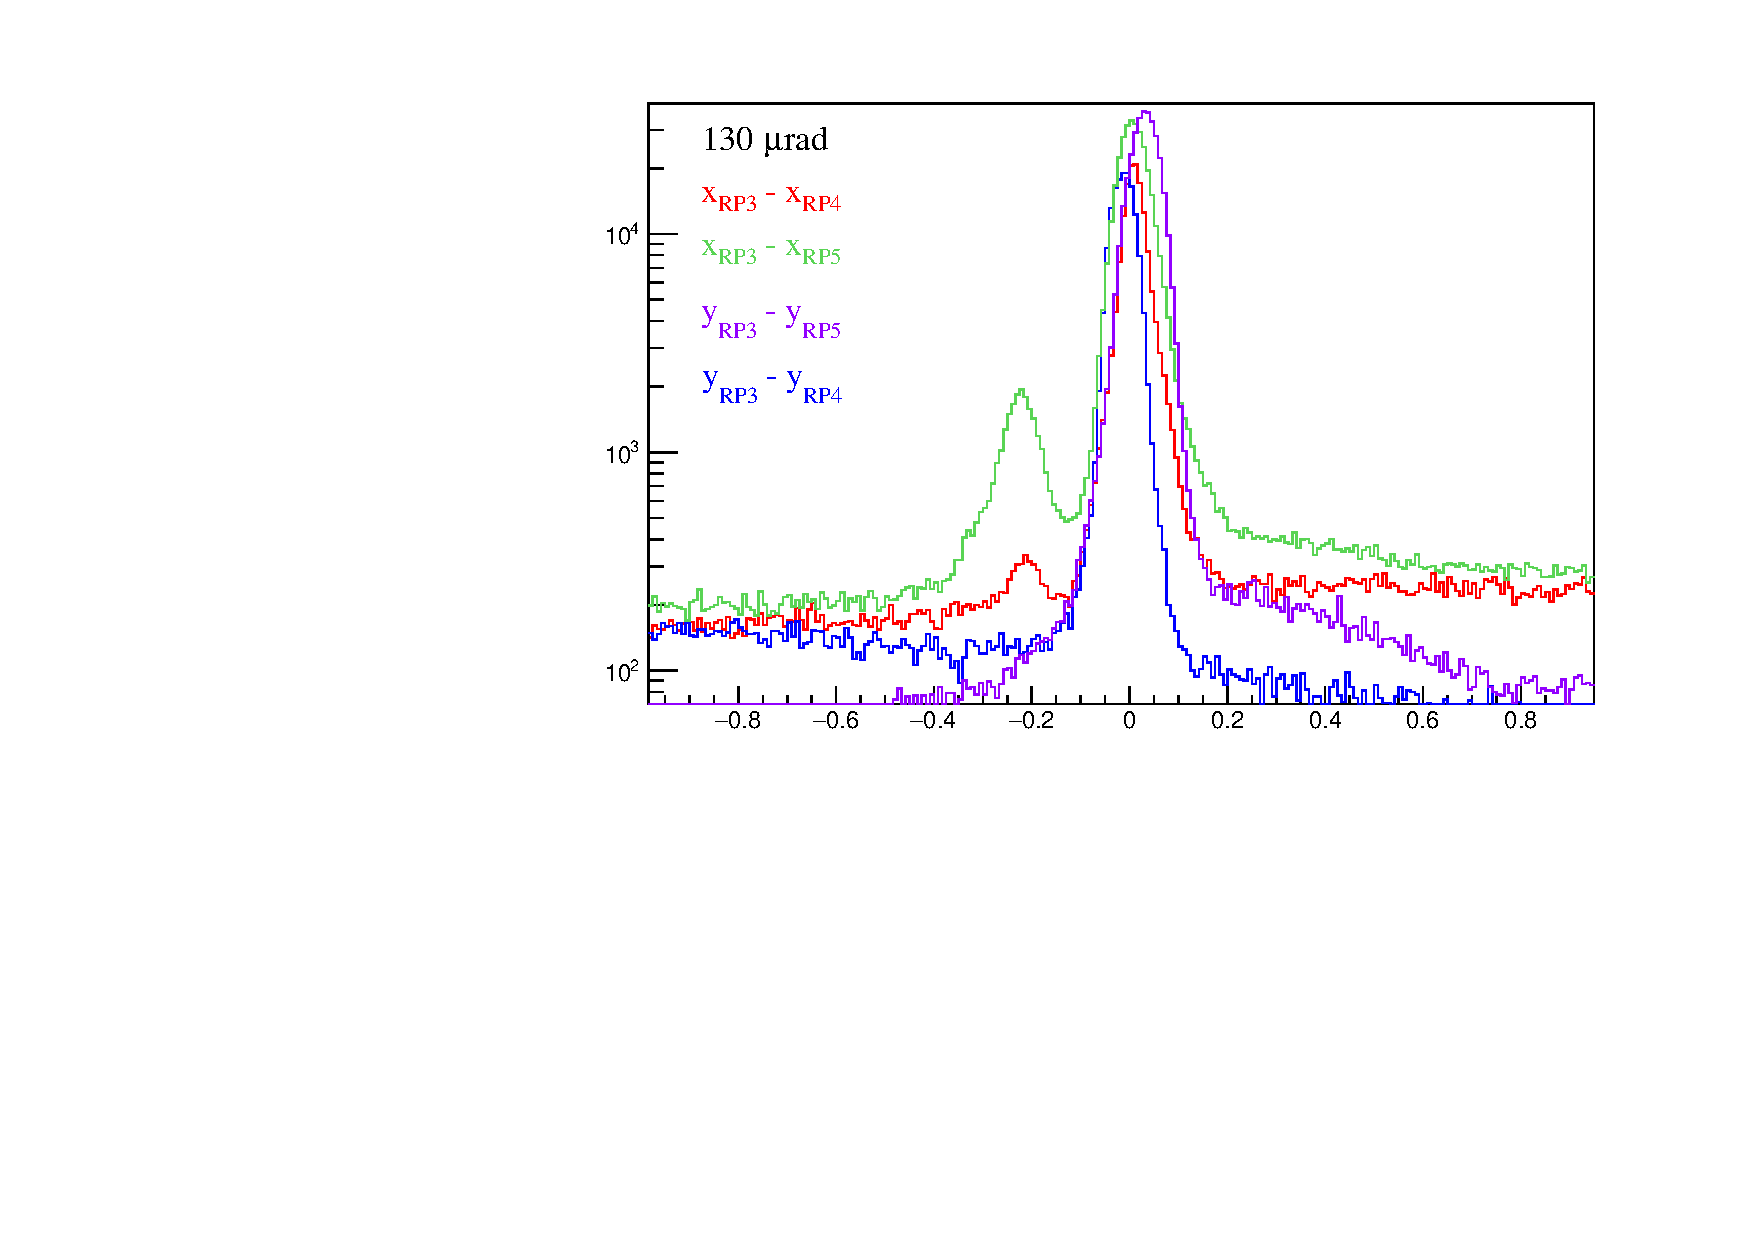
\includegraphics[width=1.0\textwidth]{130_murad_overlap.pdf}
	\end{block}
	
\end{frame}

\begin{frame}\scriptsize
	\begin{block}{Test of "absolute" alignment with elastics}
             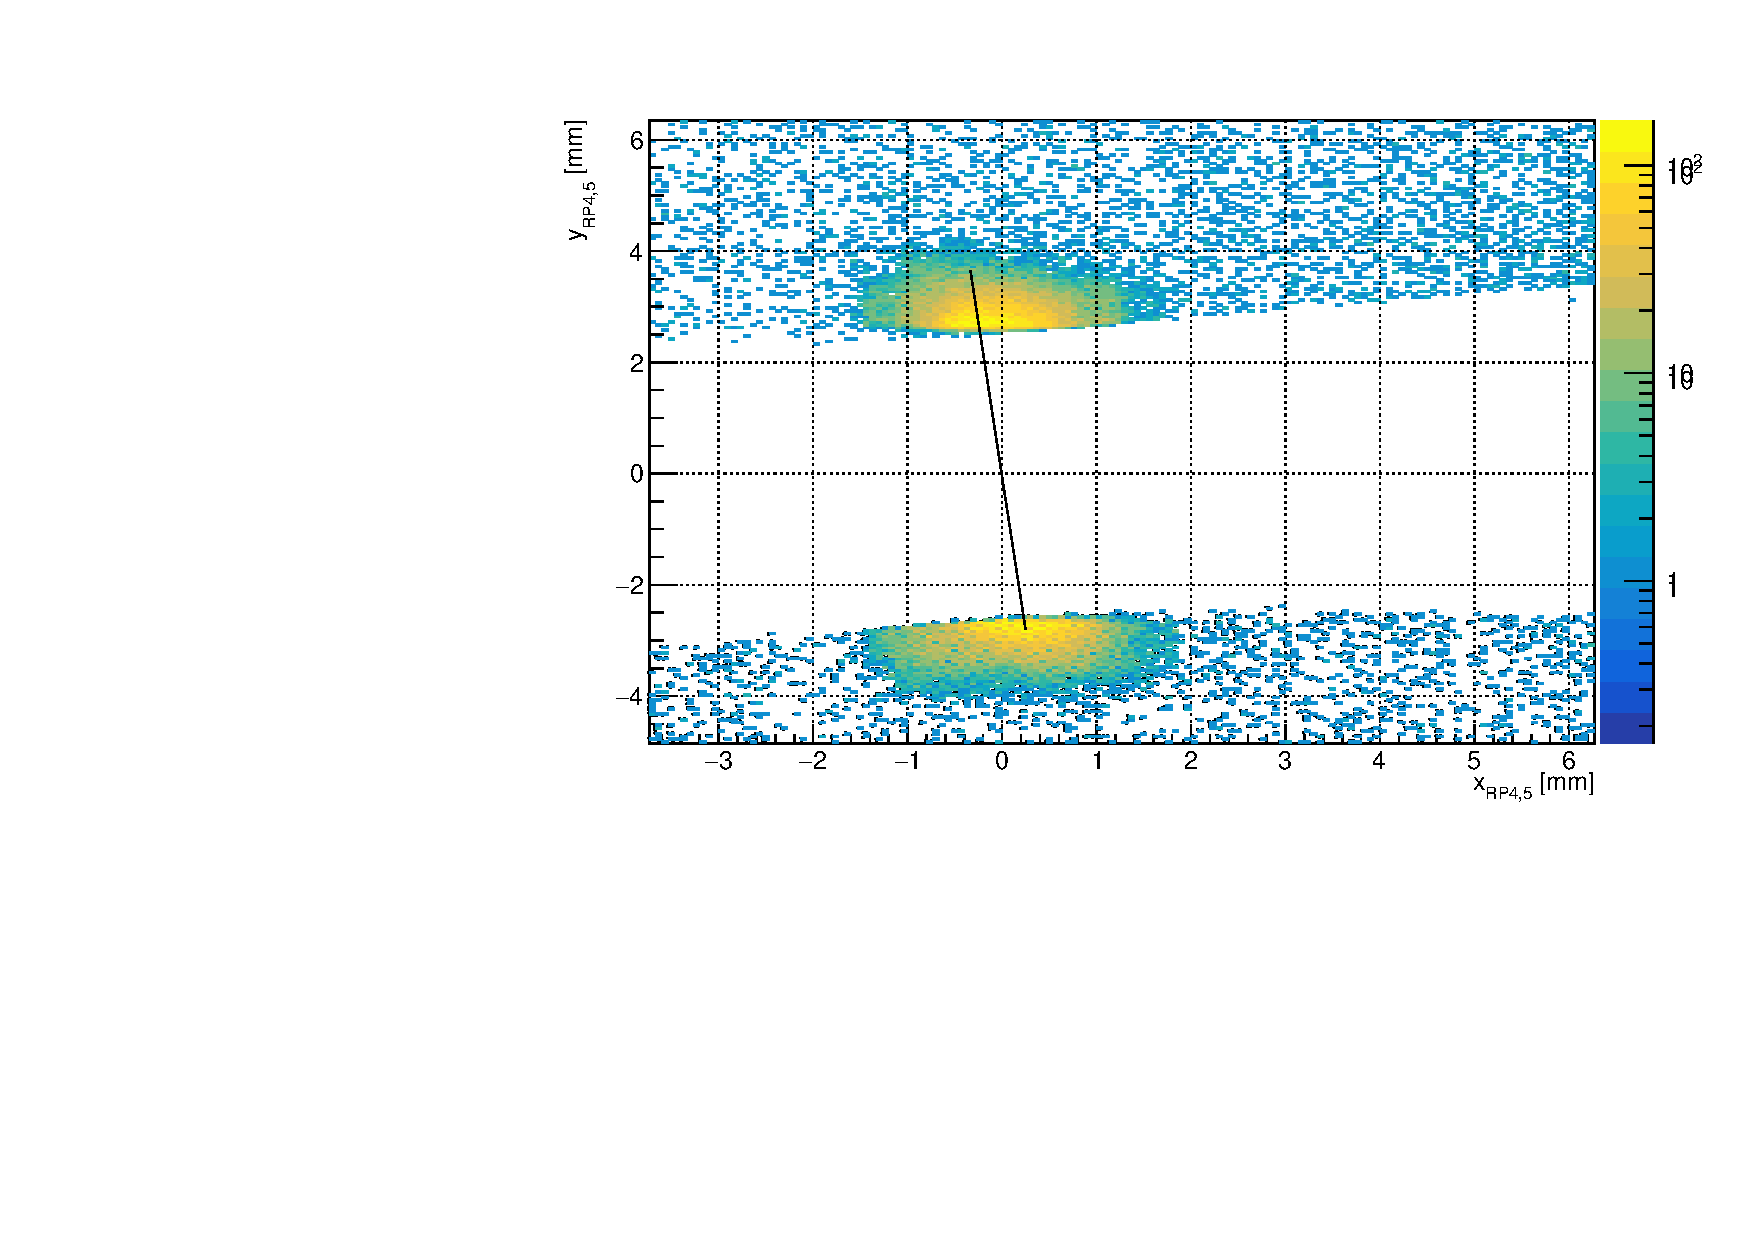
\includegraphics[width=1.0\textwidth]{elastic.pdf}
	\end{block}
	
\end{frame}

\begin{frame}
	\begin{center}
	\Large
	$x$-angle 130~$\mu$rad, $\beta^{*}=0.25$~m \\ {\small (Run 323316, 2018, September)}
	\end{center}
\end{frame}


\begin{frame}\scriptsize
	\begin{block}{The "neck" after cut}
    		\begin{itemize}
			\item Remains a bit noisy even after cut in the important range
			\item $x_{0}$ clearly below 2.5 mm
		\end{itemize}
             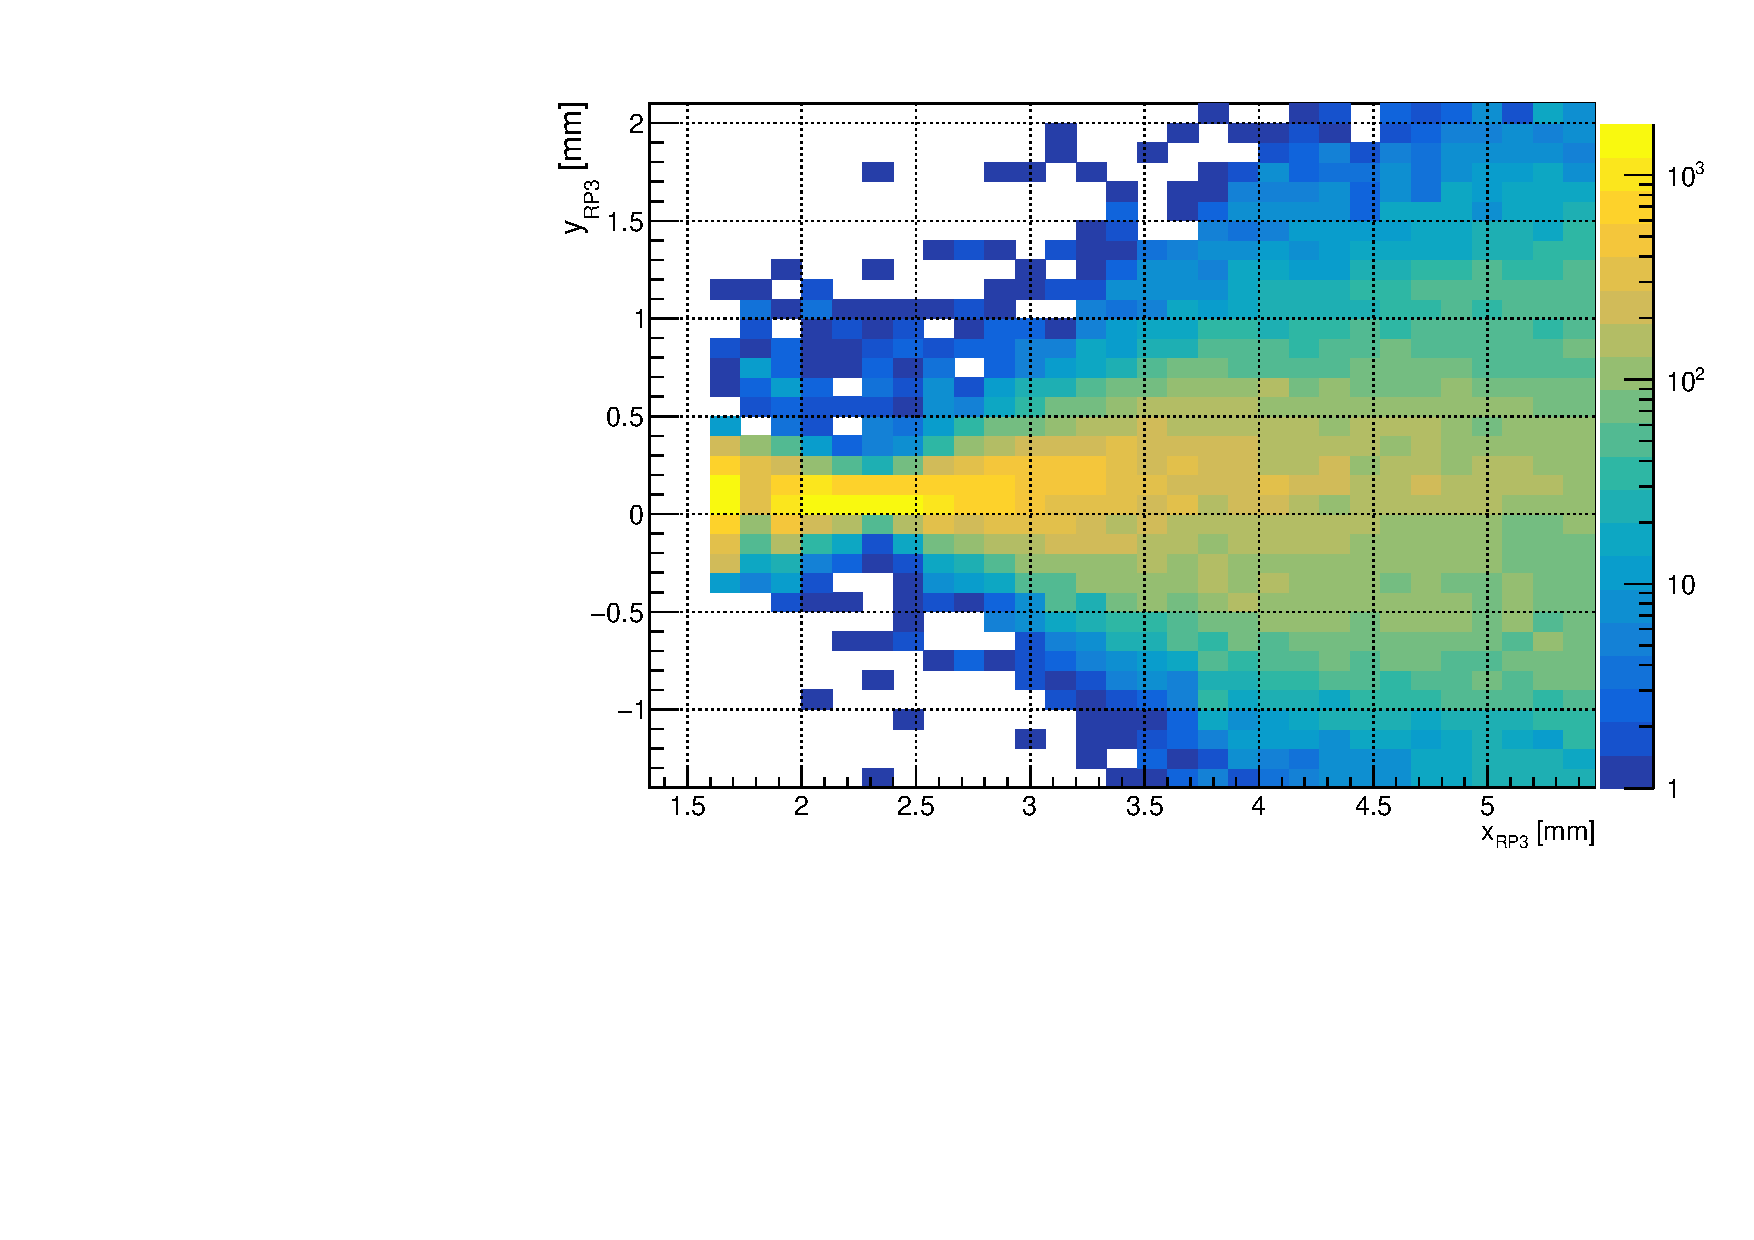
\includegraphics[width=1.0\textwidth]{Run_323316_130_murad_beta_star_0p25_m_neck.pdf}\\
	\end{block}
	
\end{frame}

\begin{frame}\scriptsize
	\begin{block}{The dx cut}
             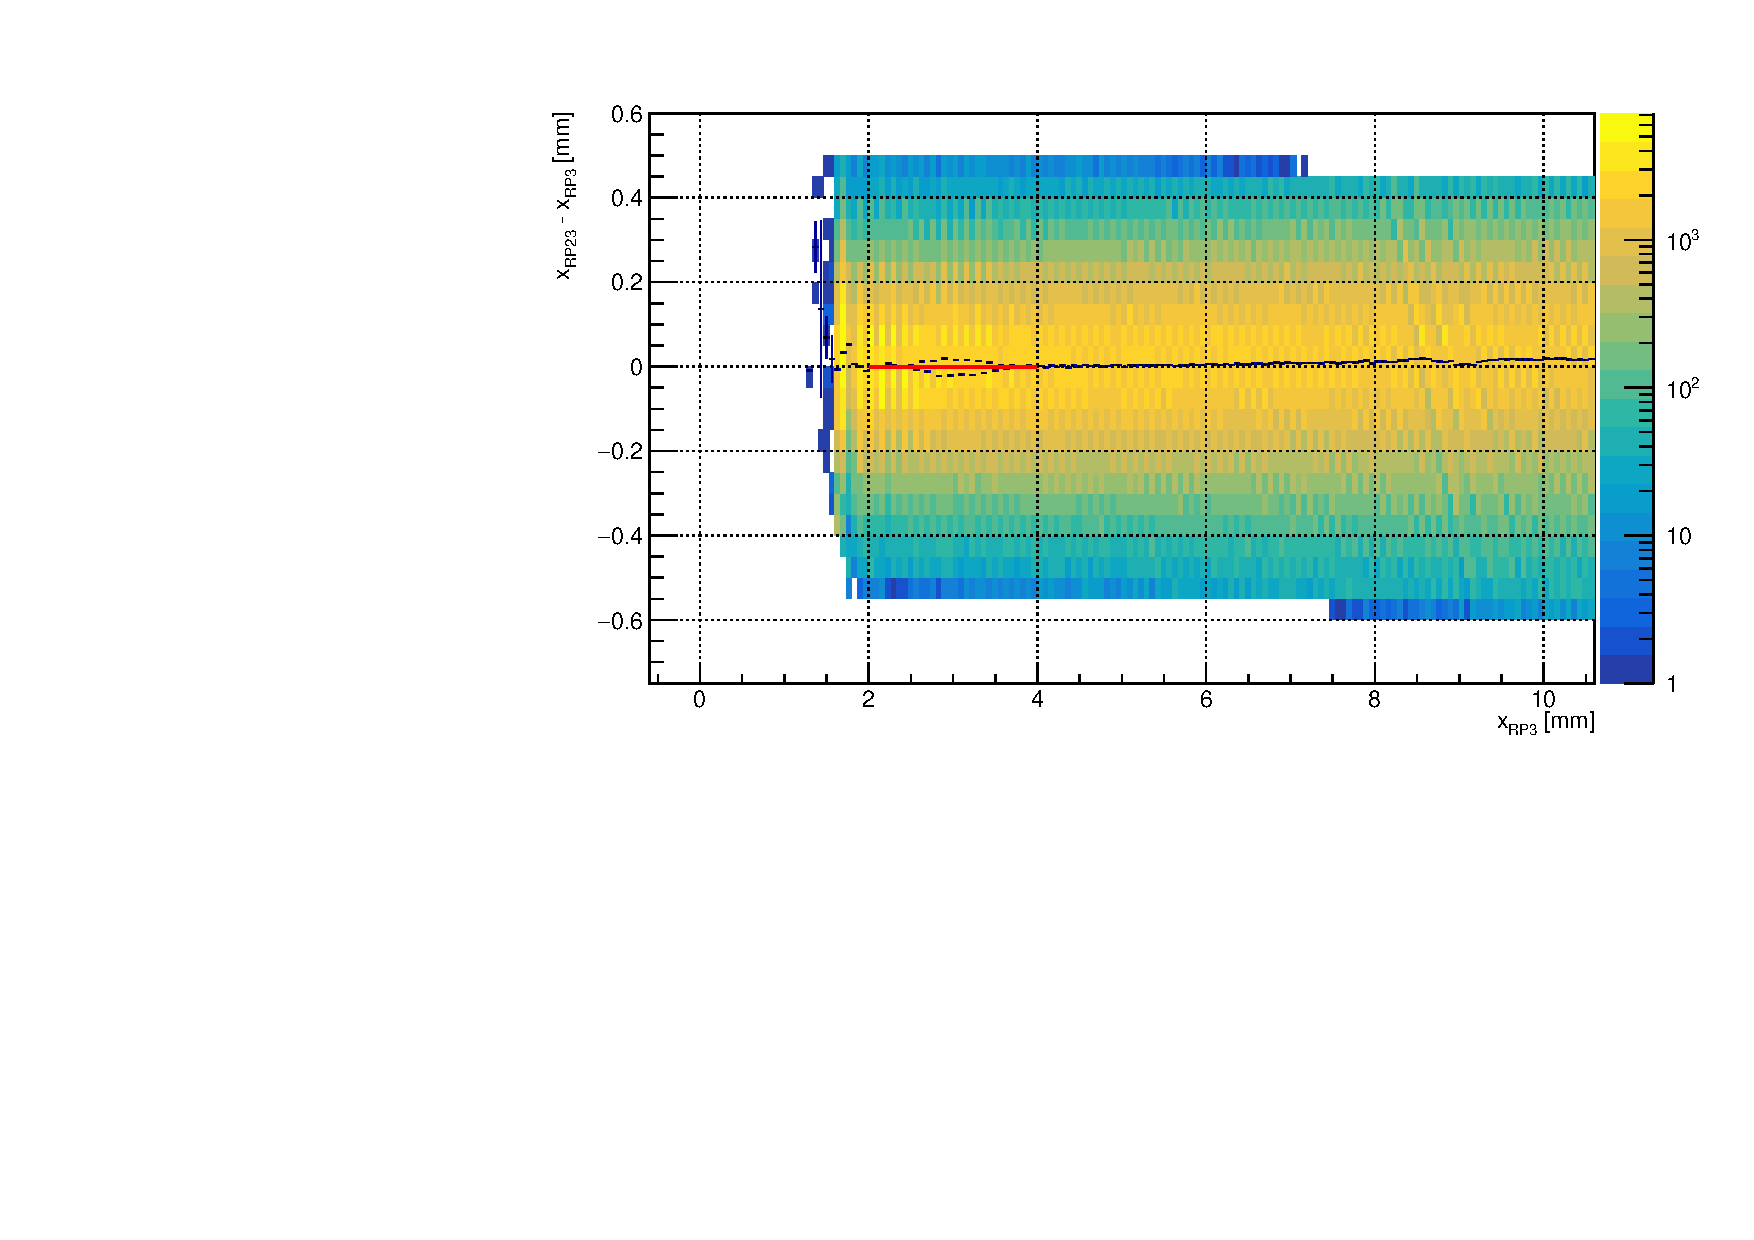
\includegraphics[width=1.0\textwidth]{Run_323316_130_murad_beta_star_0p25_m_deltax.pdf}\\
	\end{block}
	
\end{frame}

\begin{frame}\scriptsize
	\begin{block}{The $x_{0}$ point}
    		\begin{itemize}
			\item $x_{0}$ seems to be 7~\% lower than in April
			\item Alignment, optics, resolution, $x$-angle ?
		\end{itemize}

        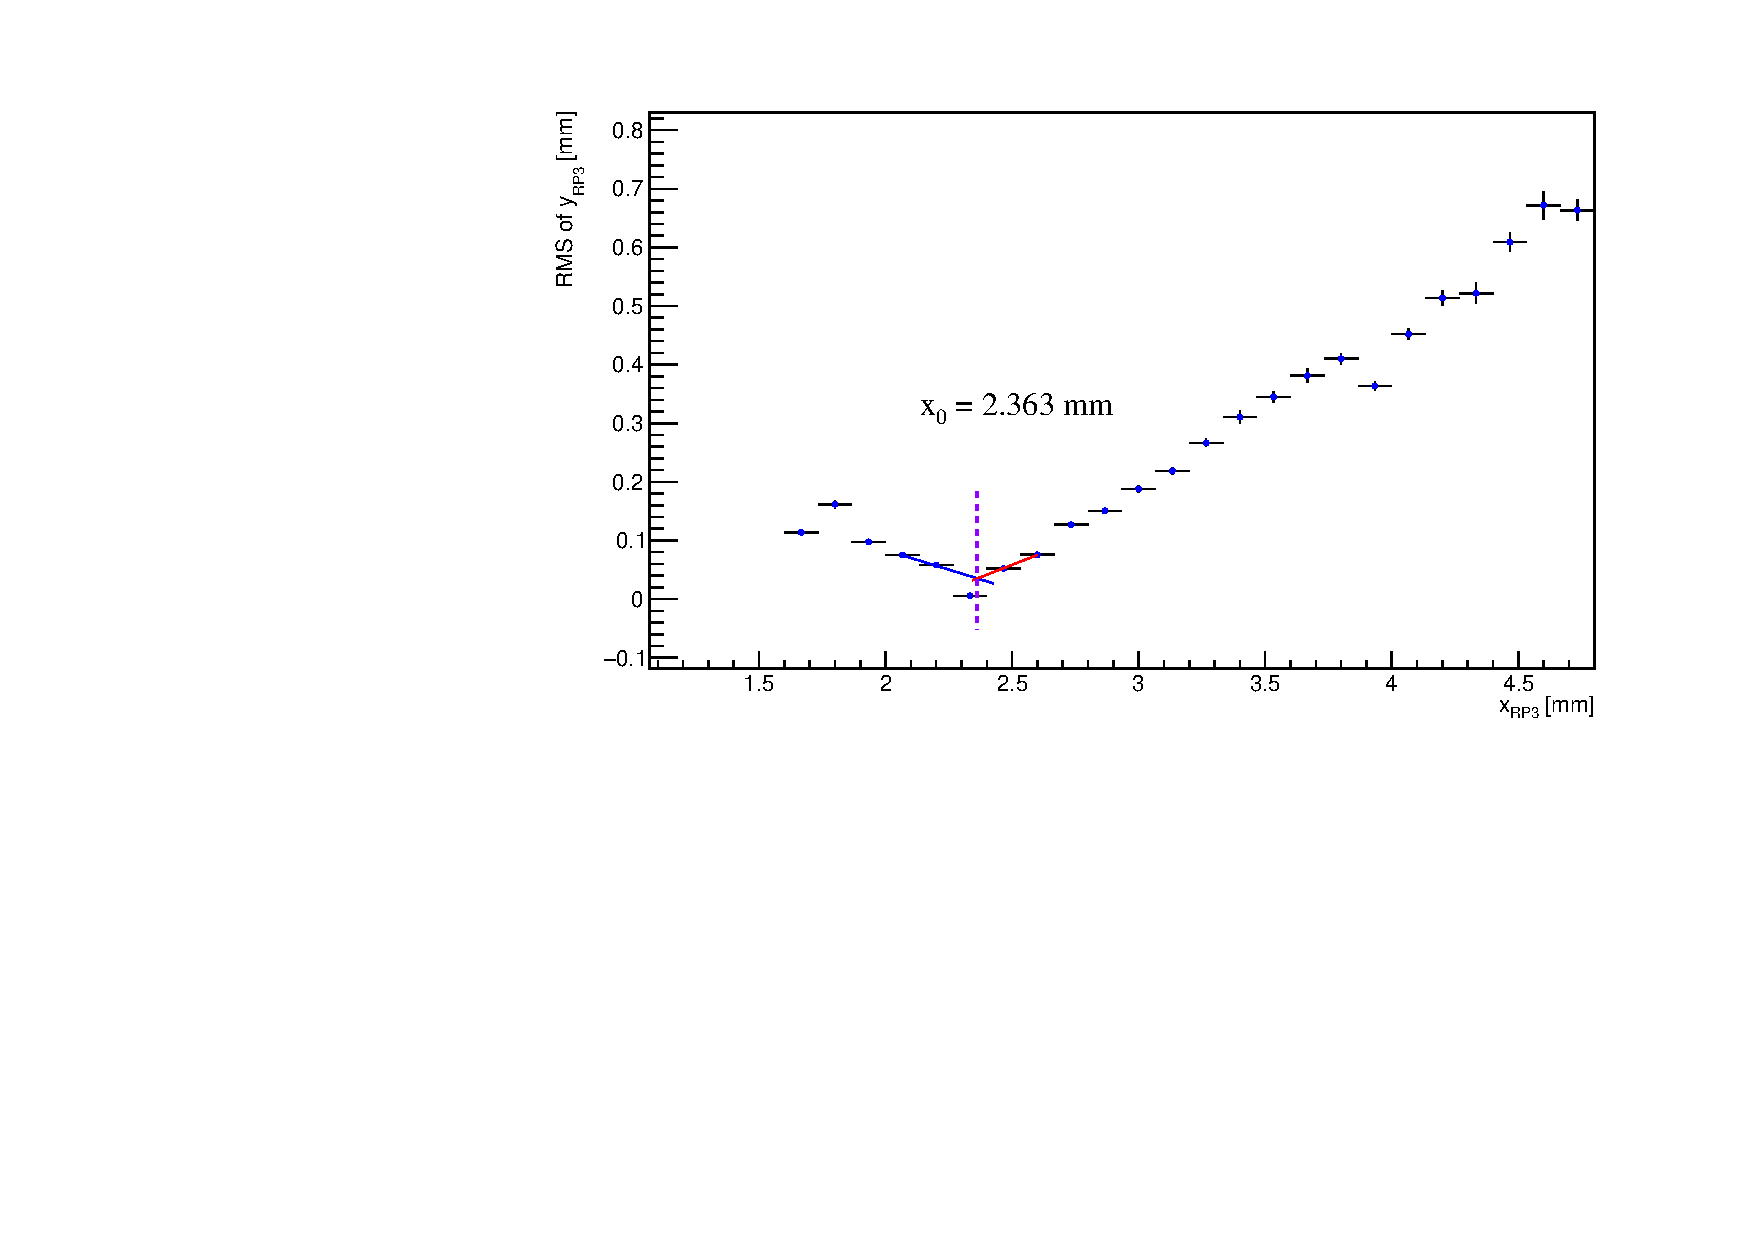
\includegraphics[width=1.0\textwidth]{Run_323316_130_murad_beta_star_0p25_m/min2.pdf}\\
	\end{block}
	
\end{frame}

\begin{frame}\scriptsize
	\begin{block}{The absolute alignment}
    		\begin{itemize}
			\item Ok, even with TProfiles 
			\item Common in events in RP 3, 4, 5 are also Ok
		\end{itemize}
             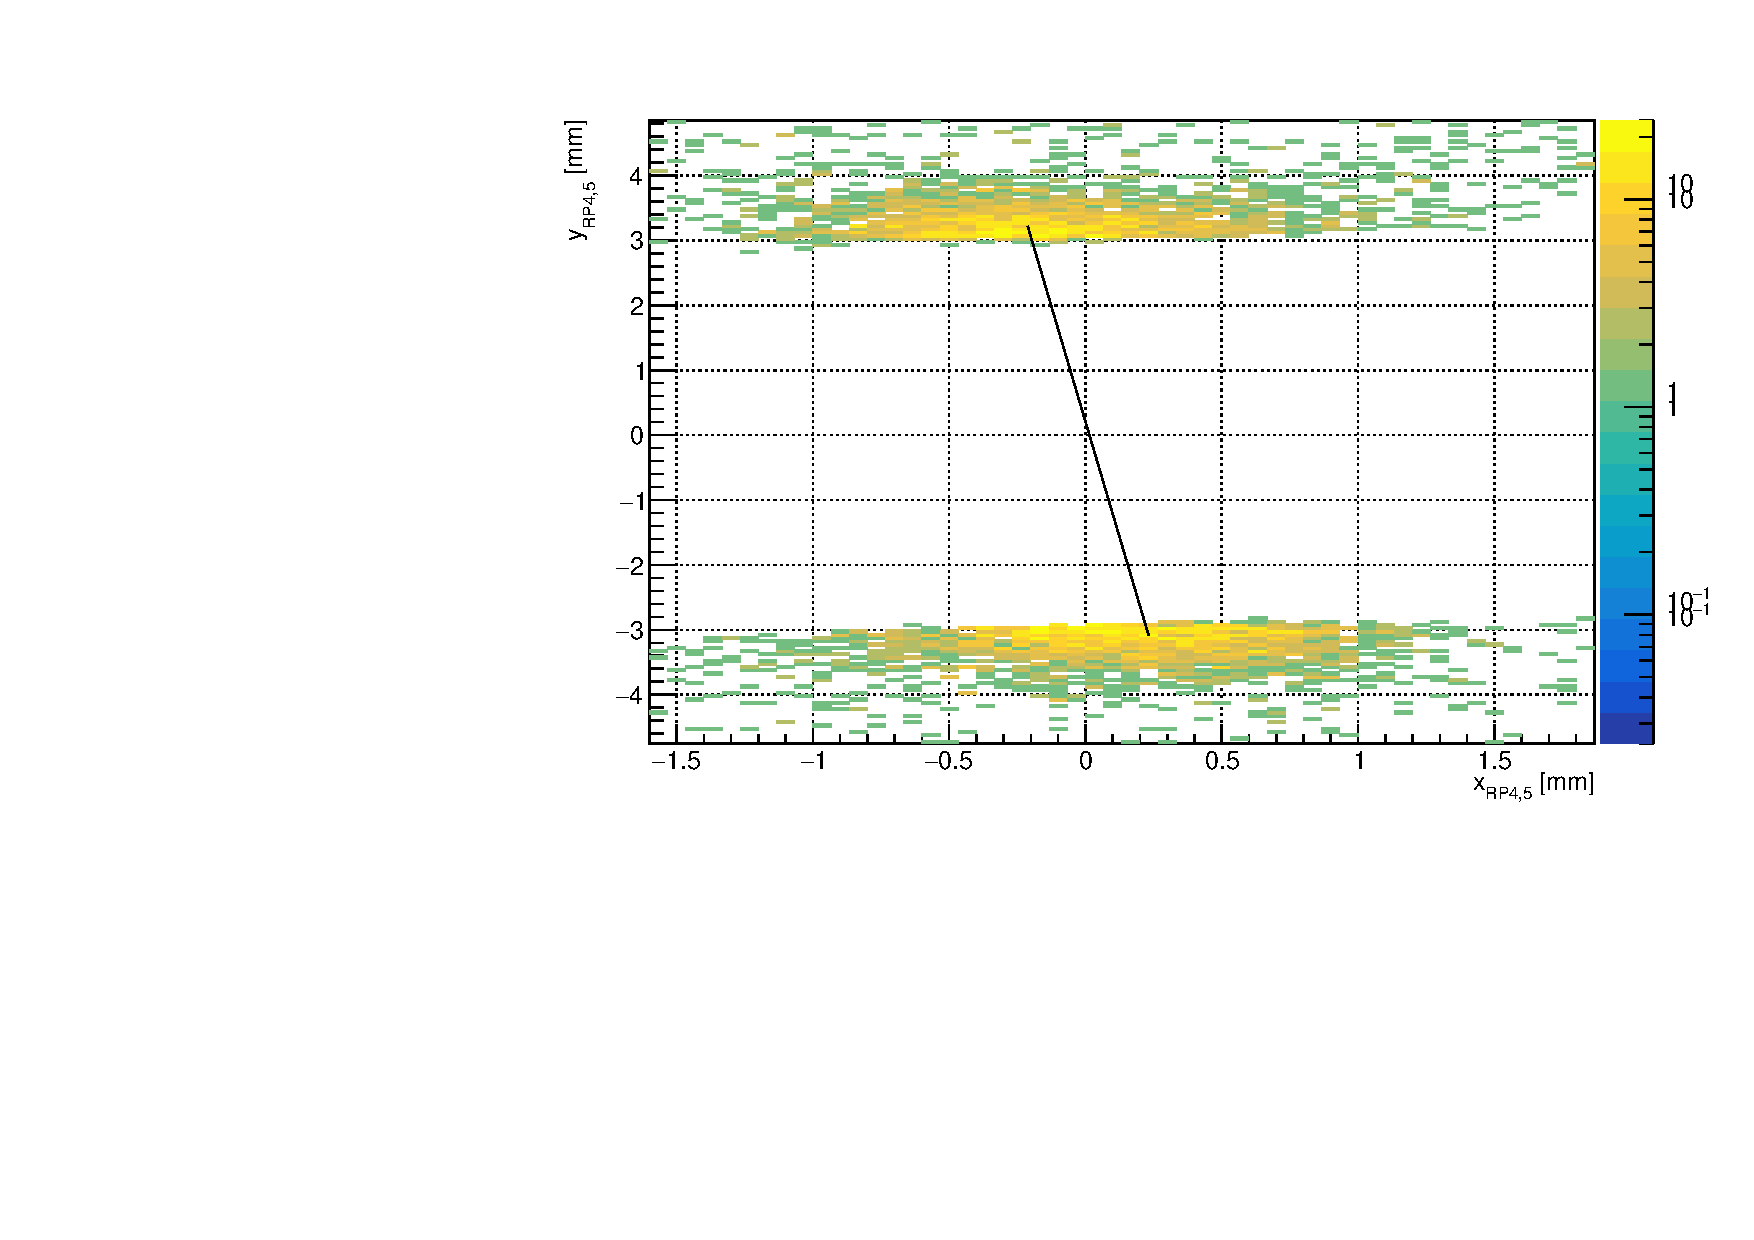
\includegraphics[width=1.0\textwidth]{Run_323316_130_murad_beta_star_0p25_m/elastic_for_meeting.pdf}\\
	\end{block}
	
\end{frame}

\begin{frame}\scriptsize
	\begin{block}{The vertical effective length $L_{y}$}
    		\begin{itemize}
			\item Ok
		\end{itemize}
             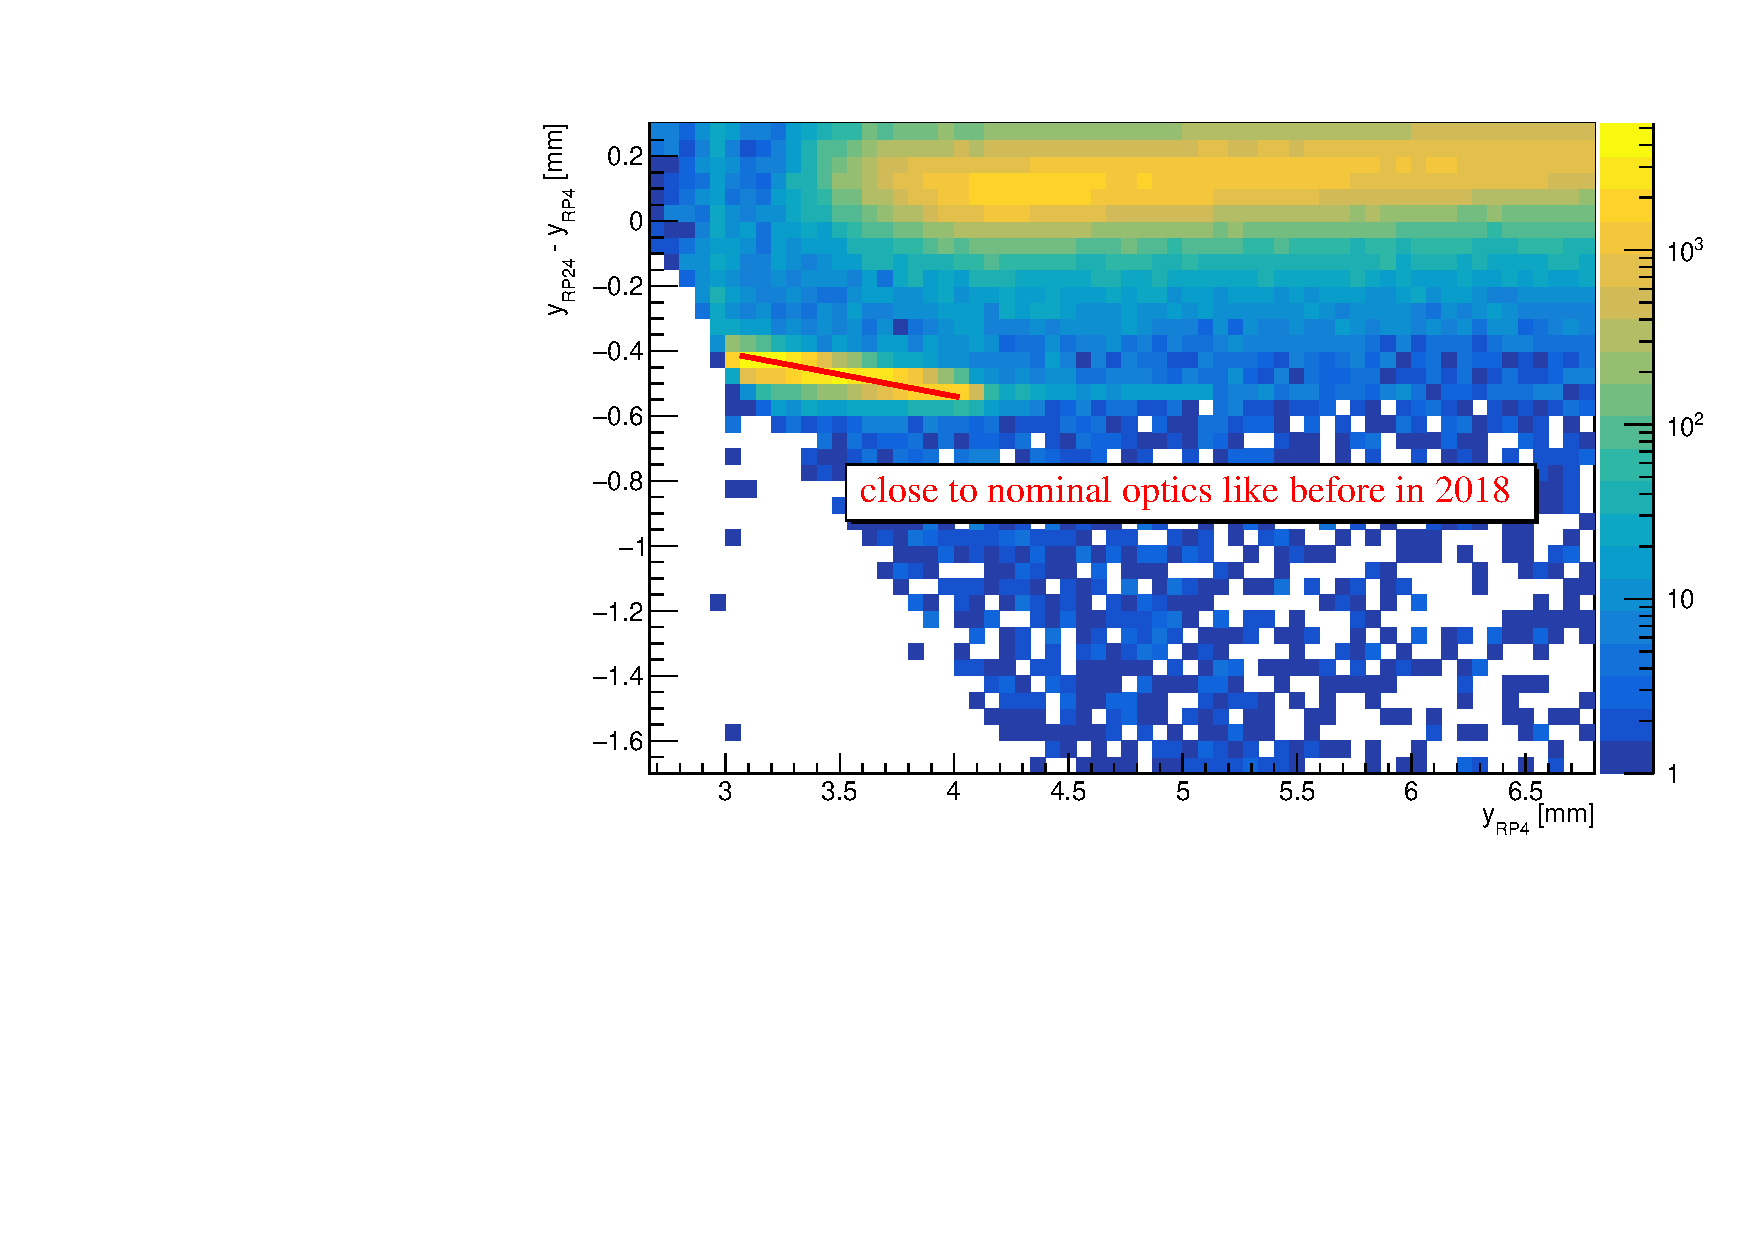
\includegraphics[width=1.0\textwidth]{Run_323316_130_murad_beta_star_0p25_m/optics_constraint_2018.pdf}\\
	\end{block}
	
\end{frame}


\begin{frame}
	\begin{center}
	\Large
	$x$-angle 130~$\mu$rad, $\beta^{*}=0.27$~m \\ {\small (Run 323311, 2018, September)}
	\end{center}
\end{frame}

\begin{frame}\scriptsize
	\begin{block}{The $x_{0}$ point}
    		\begin{itemize}
			\item Ok
		\end{itemize}
             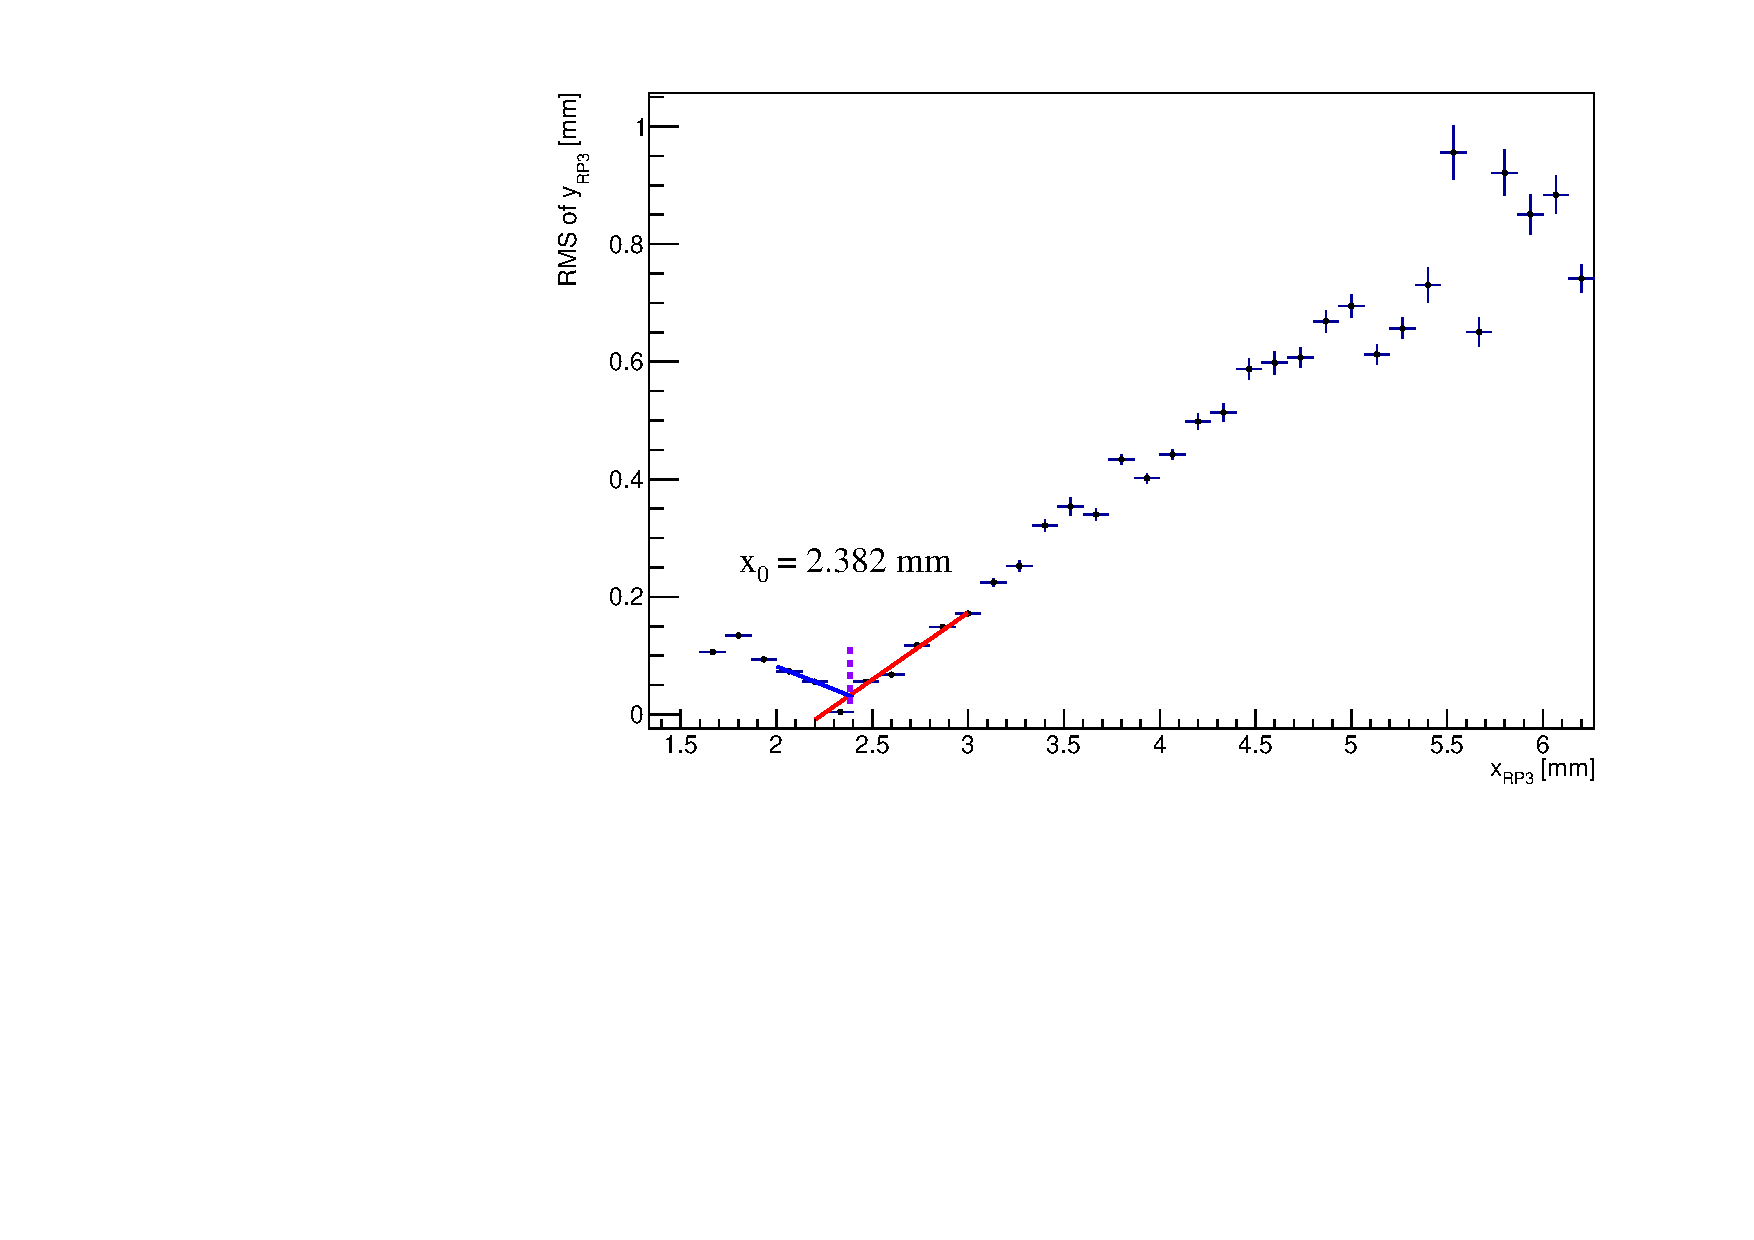
\includegraphics[width=1.0\textwidth]{Run_323311_130_murad_beta_star_0p27_m/min.pdf}\\
	\end{block}
	
\end{frame}

\begin{frame}\scriptsize
	\begin{block}{Absolute alignment and the $x_{0}$ point}
    		\begin{itemize}
			\item $x_{0}\approx$ 2.382 mm + 0.06 mm= 2.442 mm
		\end{itemize}
             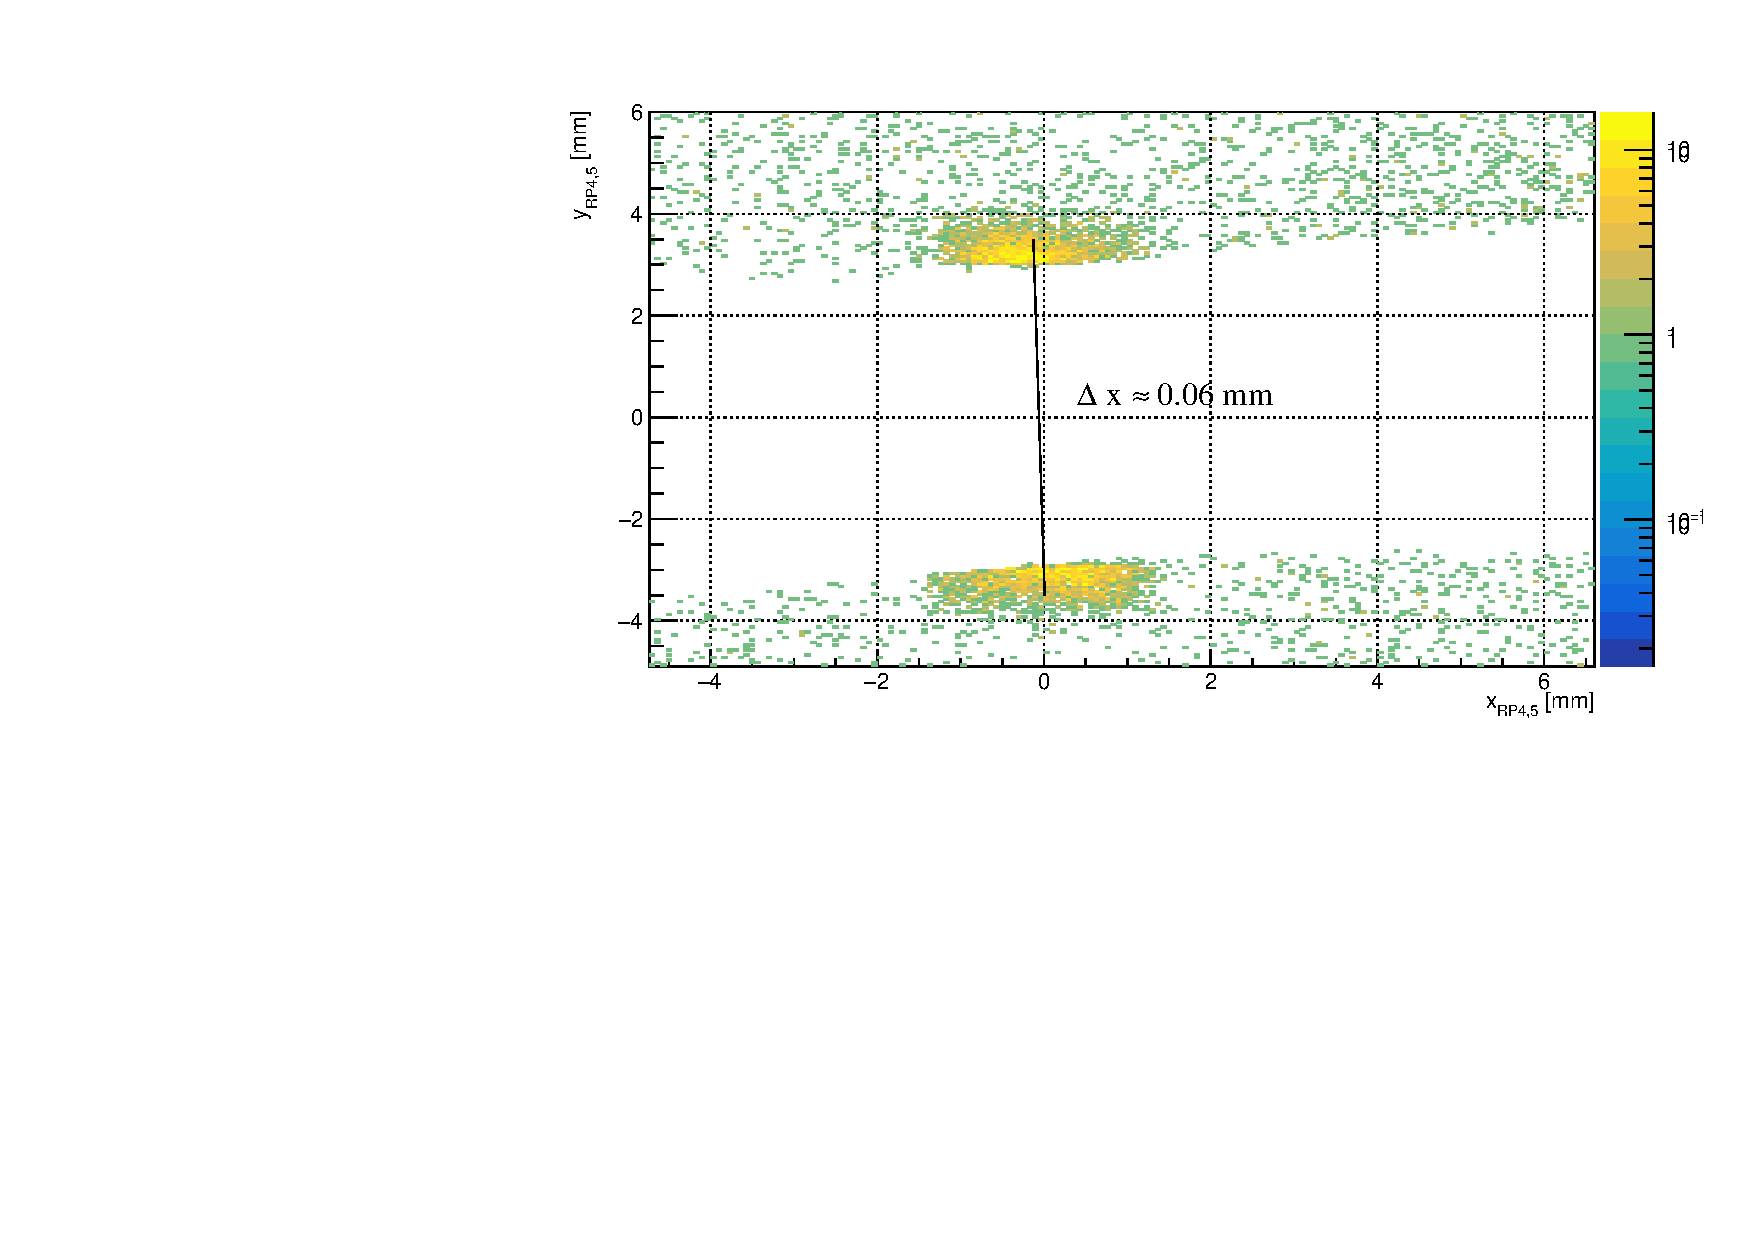
\includegraphics[width=0.7\textwidth]{Run_323311_130_murad_beta_star_0p27_m/elastic_for_meeting.pdf}\\
	\end{block}

	\begin{block}{Summary of April and September}
    		\begin{itemize}
			\item $130~\mu$rad: $x_{0}\approx 2.445$ mm $\pm$ 0.08
			\item $160~\mu$rad: $x_{0}\approx 2.10$ mm
		\end{itemize}
	\end{block}
	
\end{frame}


\begin{frame}
	\begin{center}
	\Large {\color{blue} Right arm}\\
	$x$-angle 130~$\mu$rad, $\beta^{*}=0.25$ m\\ {\small (Run 314276, 2018, April)}
	\end{center}
\end{frame}

\begin{frame}\scriptsize
	\begin{block}{The $x_{0}$ point in RP103}
    		\begin{itemize}
			\item Calibration point is not visible
			\item 2017 data suggest a factor 1.298 between left and right arm
			\item $x_{0}$ "should" be around 1.883 $\pm$ 0.08
		\end{itemize}
             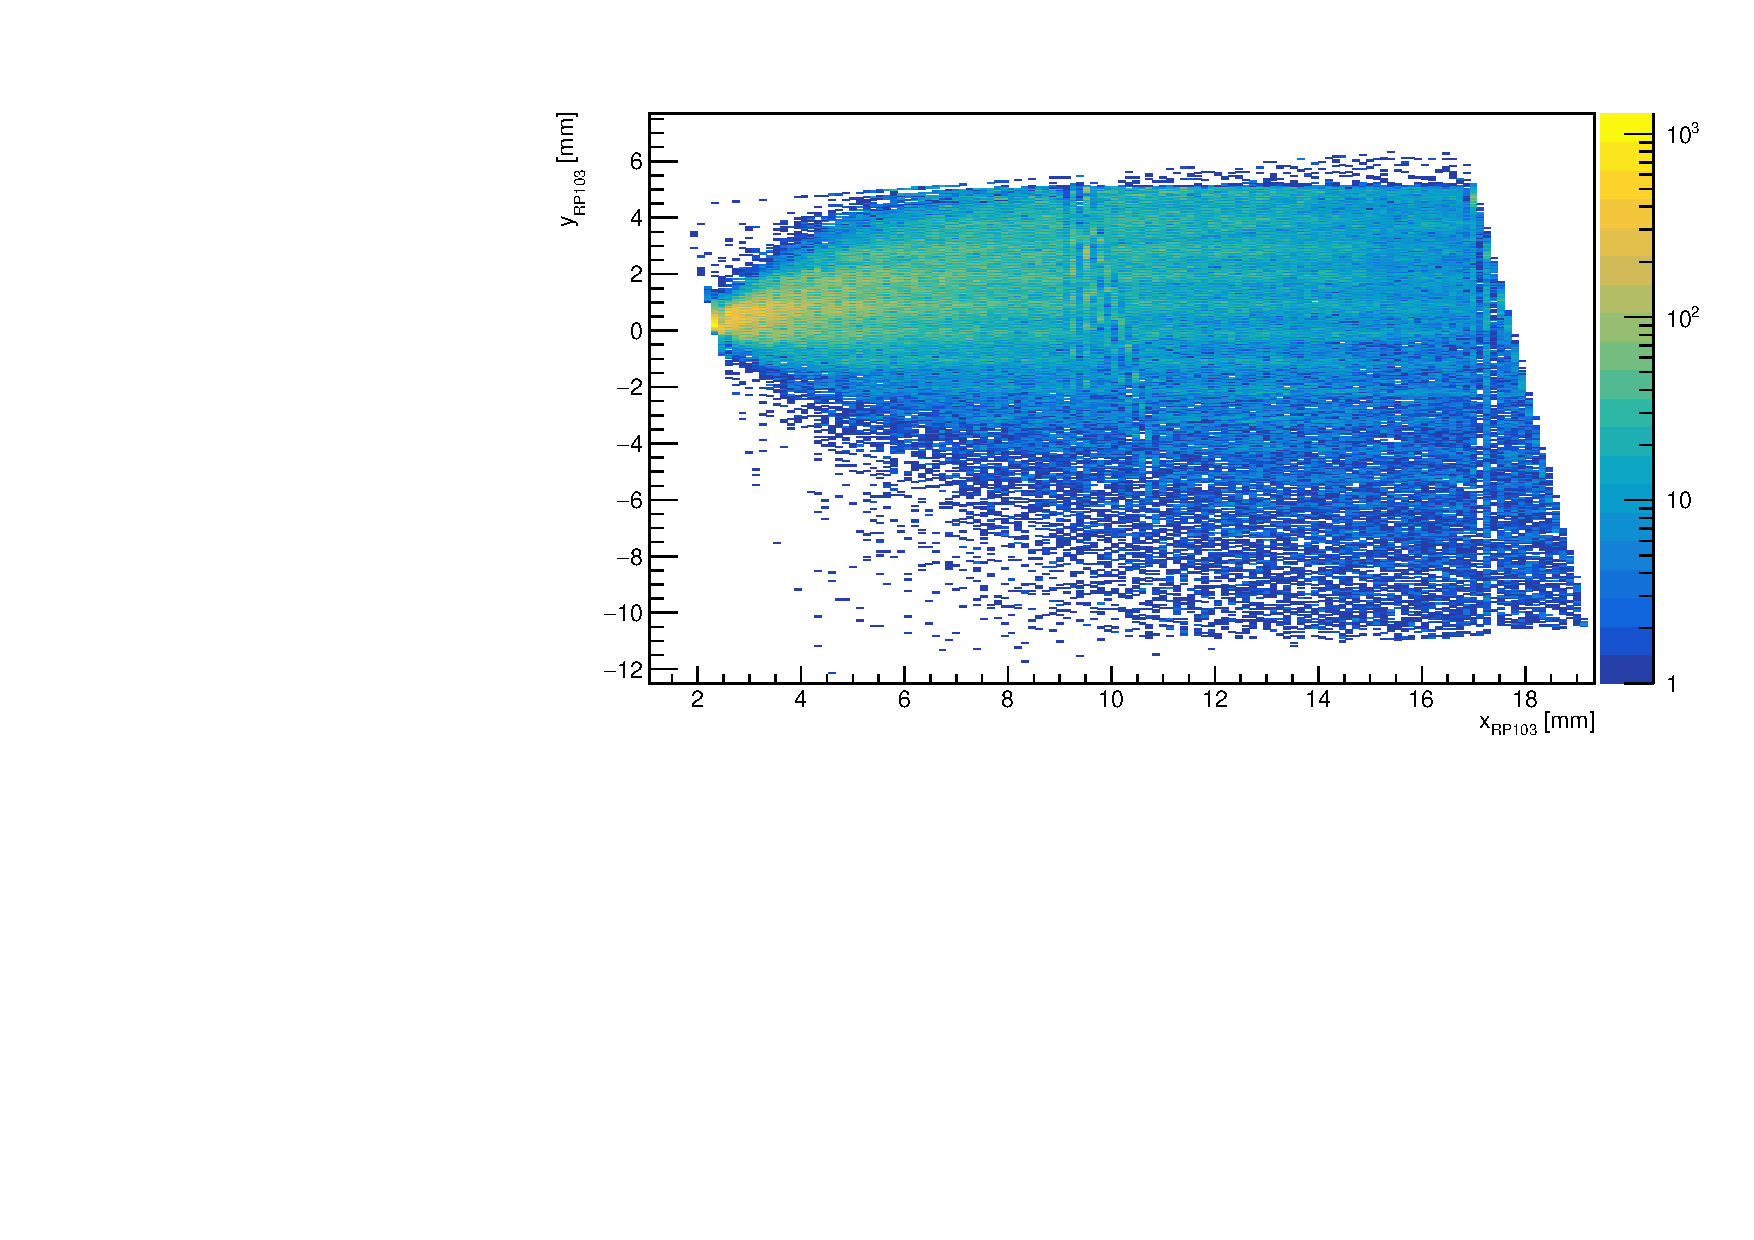
\includegraphics[width=1.0\textwidth]{Run_314276/neck_rp_103_m.pdf}
	\end{block}
	
\end{frame}

\begin{frame}\scriptsize
	\begin{block}{The $x_{0}$ point in RP103}
    		\begin{itemize}
			\item Parabolic fit
			\item First points not used, fit quality very low
			\item Extrapolation point is OK
			\item Dimuon data will help (also for left arm!)
		\end{itemize}
		\begin{center}
             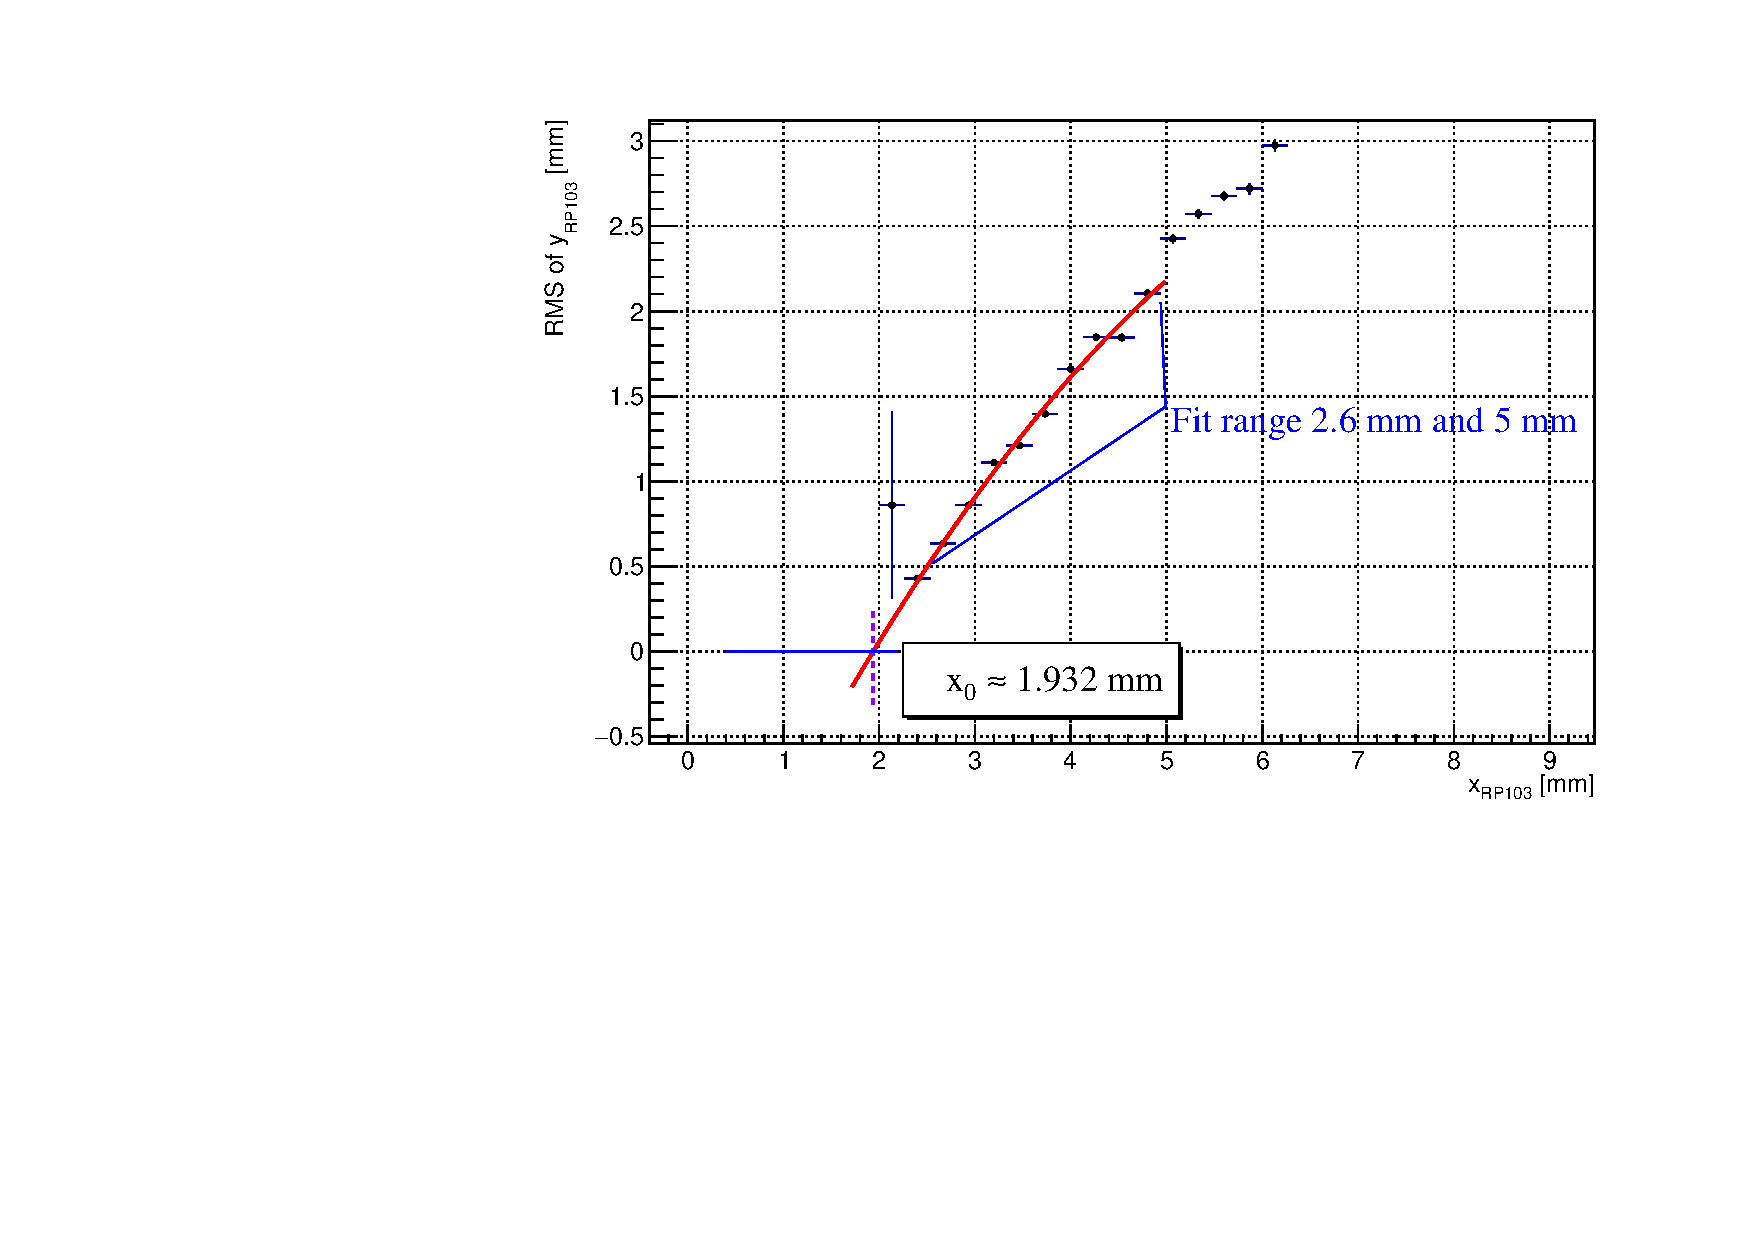
\includegraphics[width=0.8\textwidth]{Run_314276/neck_rp_103_variance_fit_meeintg.pdf}
		\end{center}
	\end{block}
	
\end{frame}

\begin{frame}\scriptsize
	\begin{block}{A curiosity in the right arm from September}
    		\begin{itemize}
			\item Reason: $L_{x}=0$ close to RP
			\item No coupling (MQSX off)
			\item Good for optics checks!
		\end{itemize}
	\begin{center}
             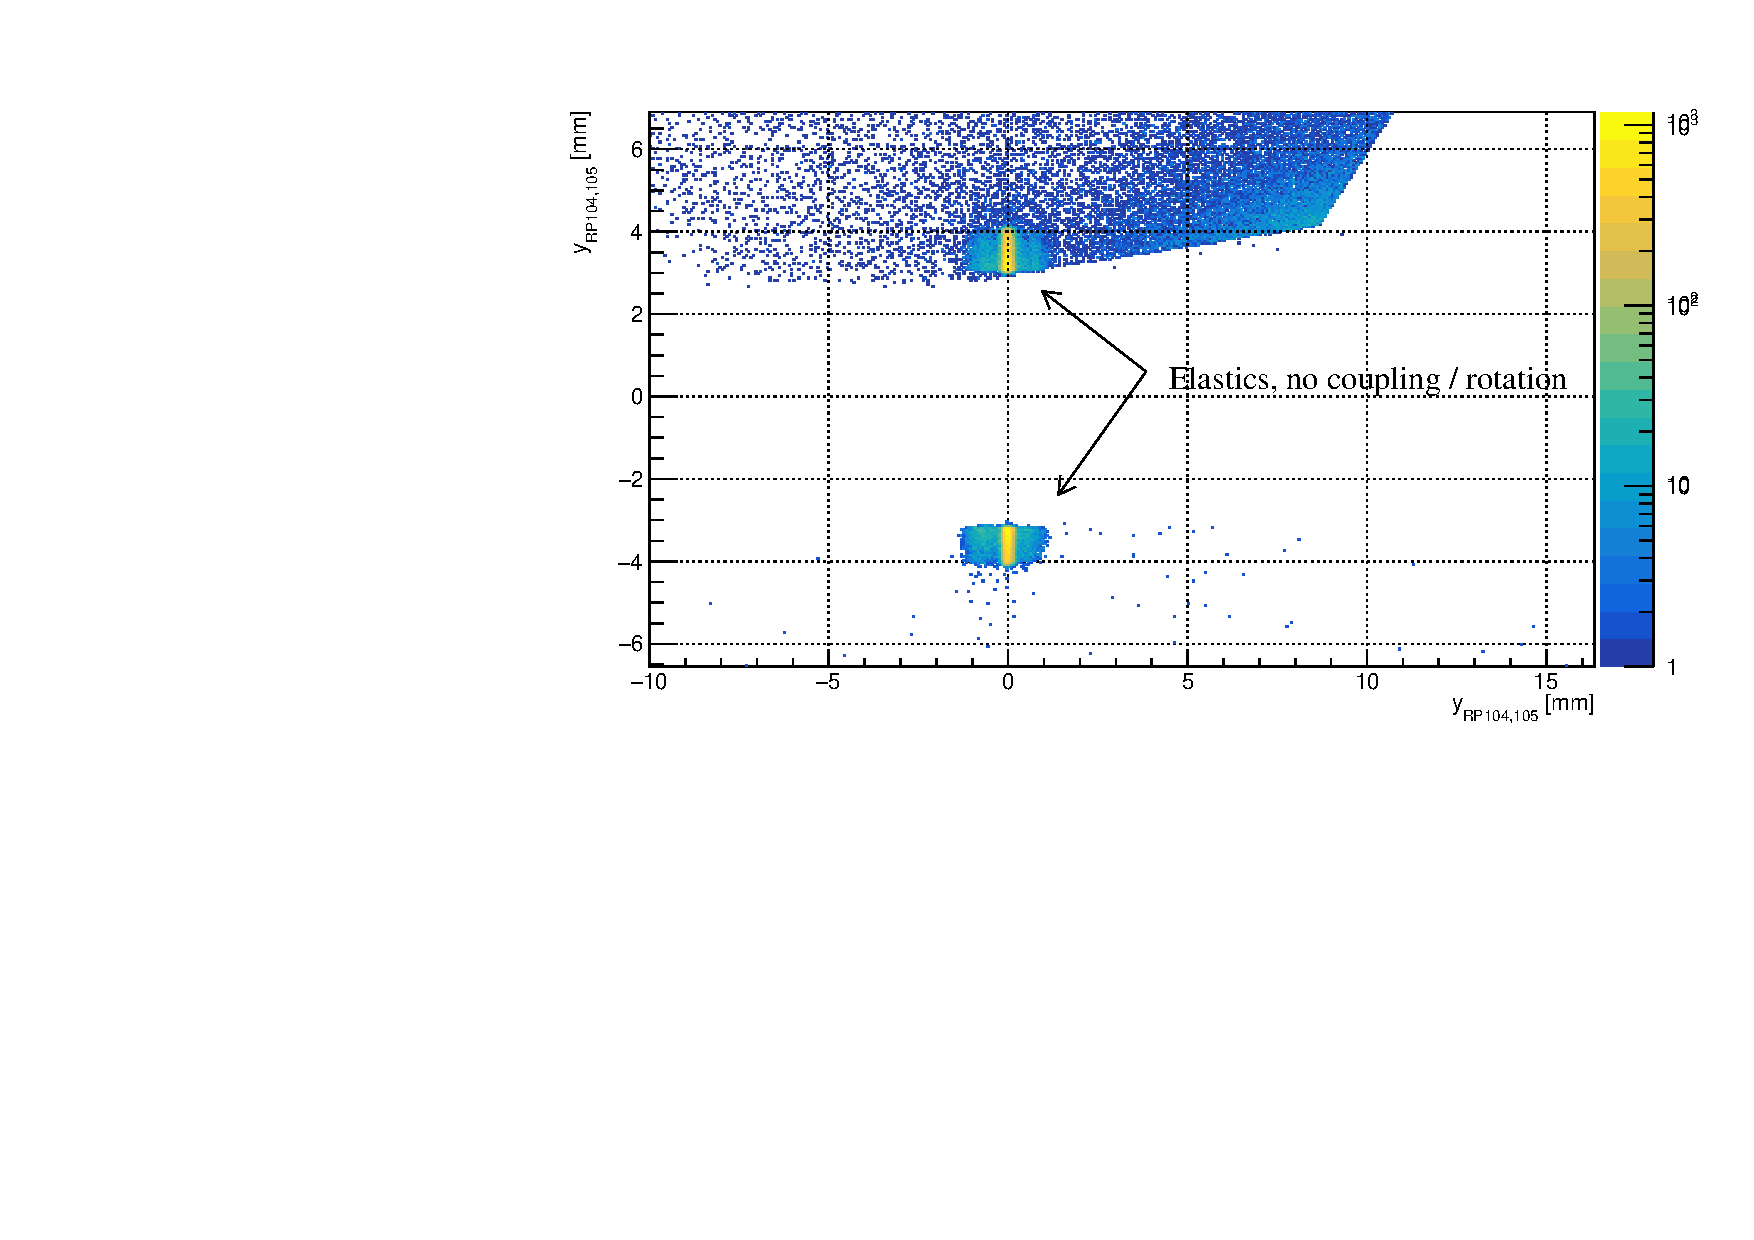
\includegraphics[width=0.48\textwidth]{RP_104_105_elastics_curiosity.pdf}\\
             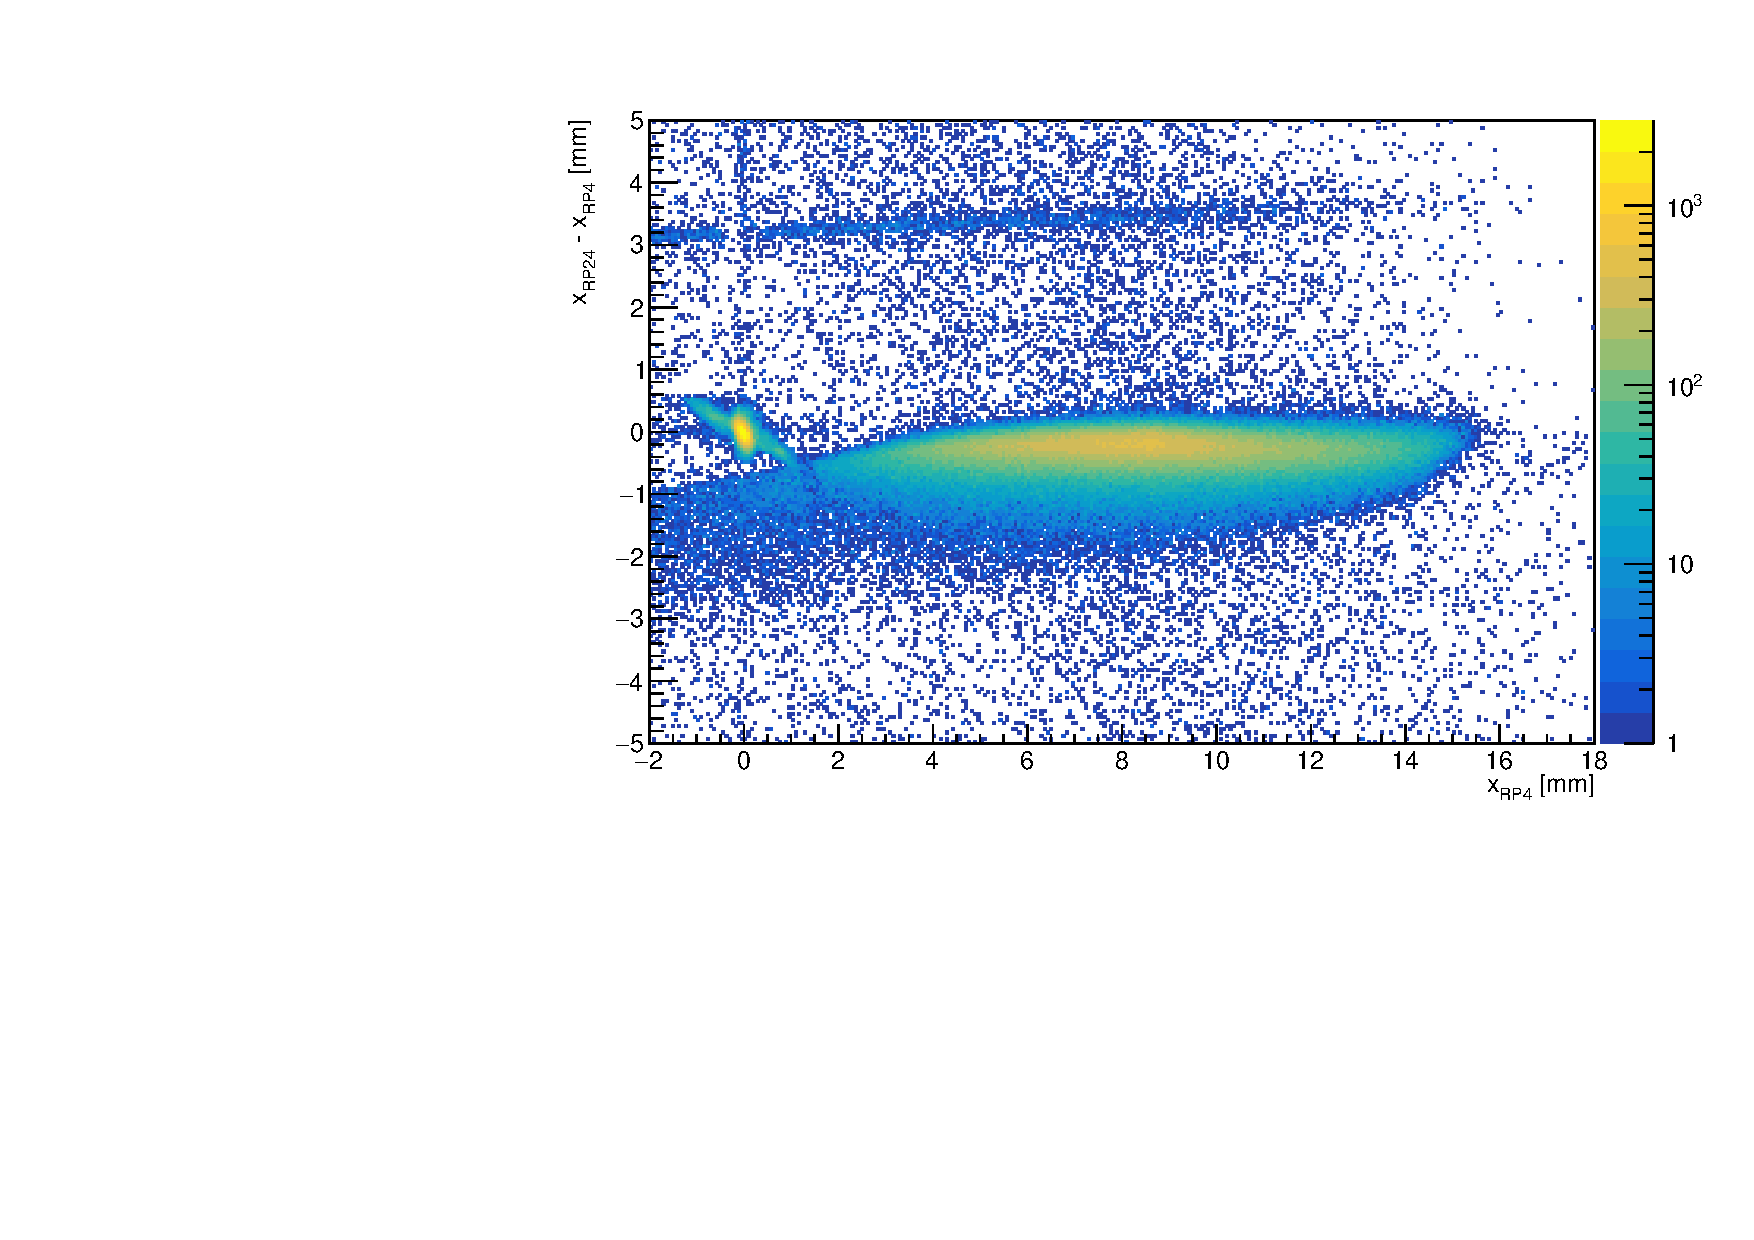
\includegraphics[width=0.48\textwidth]{x_check.pdf}
		\end{center}
	\end{block}
	
\end{frame}


\begin{frame}
	\begin{center}
	\Large
	Notes on beam divergence
	\end{center}
\end{frame}

\begin{frame}\scriptsize
	\begin{block}{Based on emittance and beam spot}
             \href{https://indico.cern.ch/event/672586/contributions/2751640/attachments/1539182/2412882/Summary.pdf}{\color{blue} \underline{\ttfamily Beam divergence study}} from CT-PPS Physics meeting
     		\begin{itemize}
			\item Lorentz $\gamma_{\rm proton}=\frac{E_{\rm beam}}{M_{\rm proton}}=\frac{6500~{\rm GeV}}{0.93827~{\rm GeV}}$
			\item $\sigma_{x,y}^{*}=\sqrt{\frac{\beta_{x,y}^{*}\cdot\epsilon}{\gamma_{\rm proton}}}=\sqrt{\frac{0.4\cdot3.5\cdot10^{-6}}{\gamma_{\rm proton}}}=14~\mu$m ($\epsilon$ stands for the emittance)
			\item The figure shows the physics run closest to the alignment run (from Jonathan)
			\item Excellent agreement between data and model
			\item Page 6: beam divergence $\sigma(x')^{*}=\sigma(x)^{*}/\beta^{*}=14~\mu m / 0.4 m=35~\mu rad$ 
		\end{itemize}
		\begin{figure}
			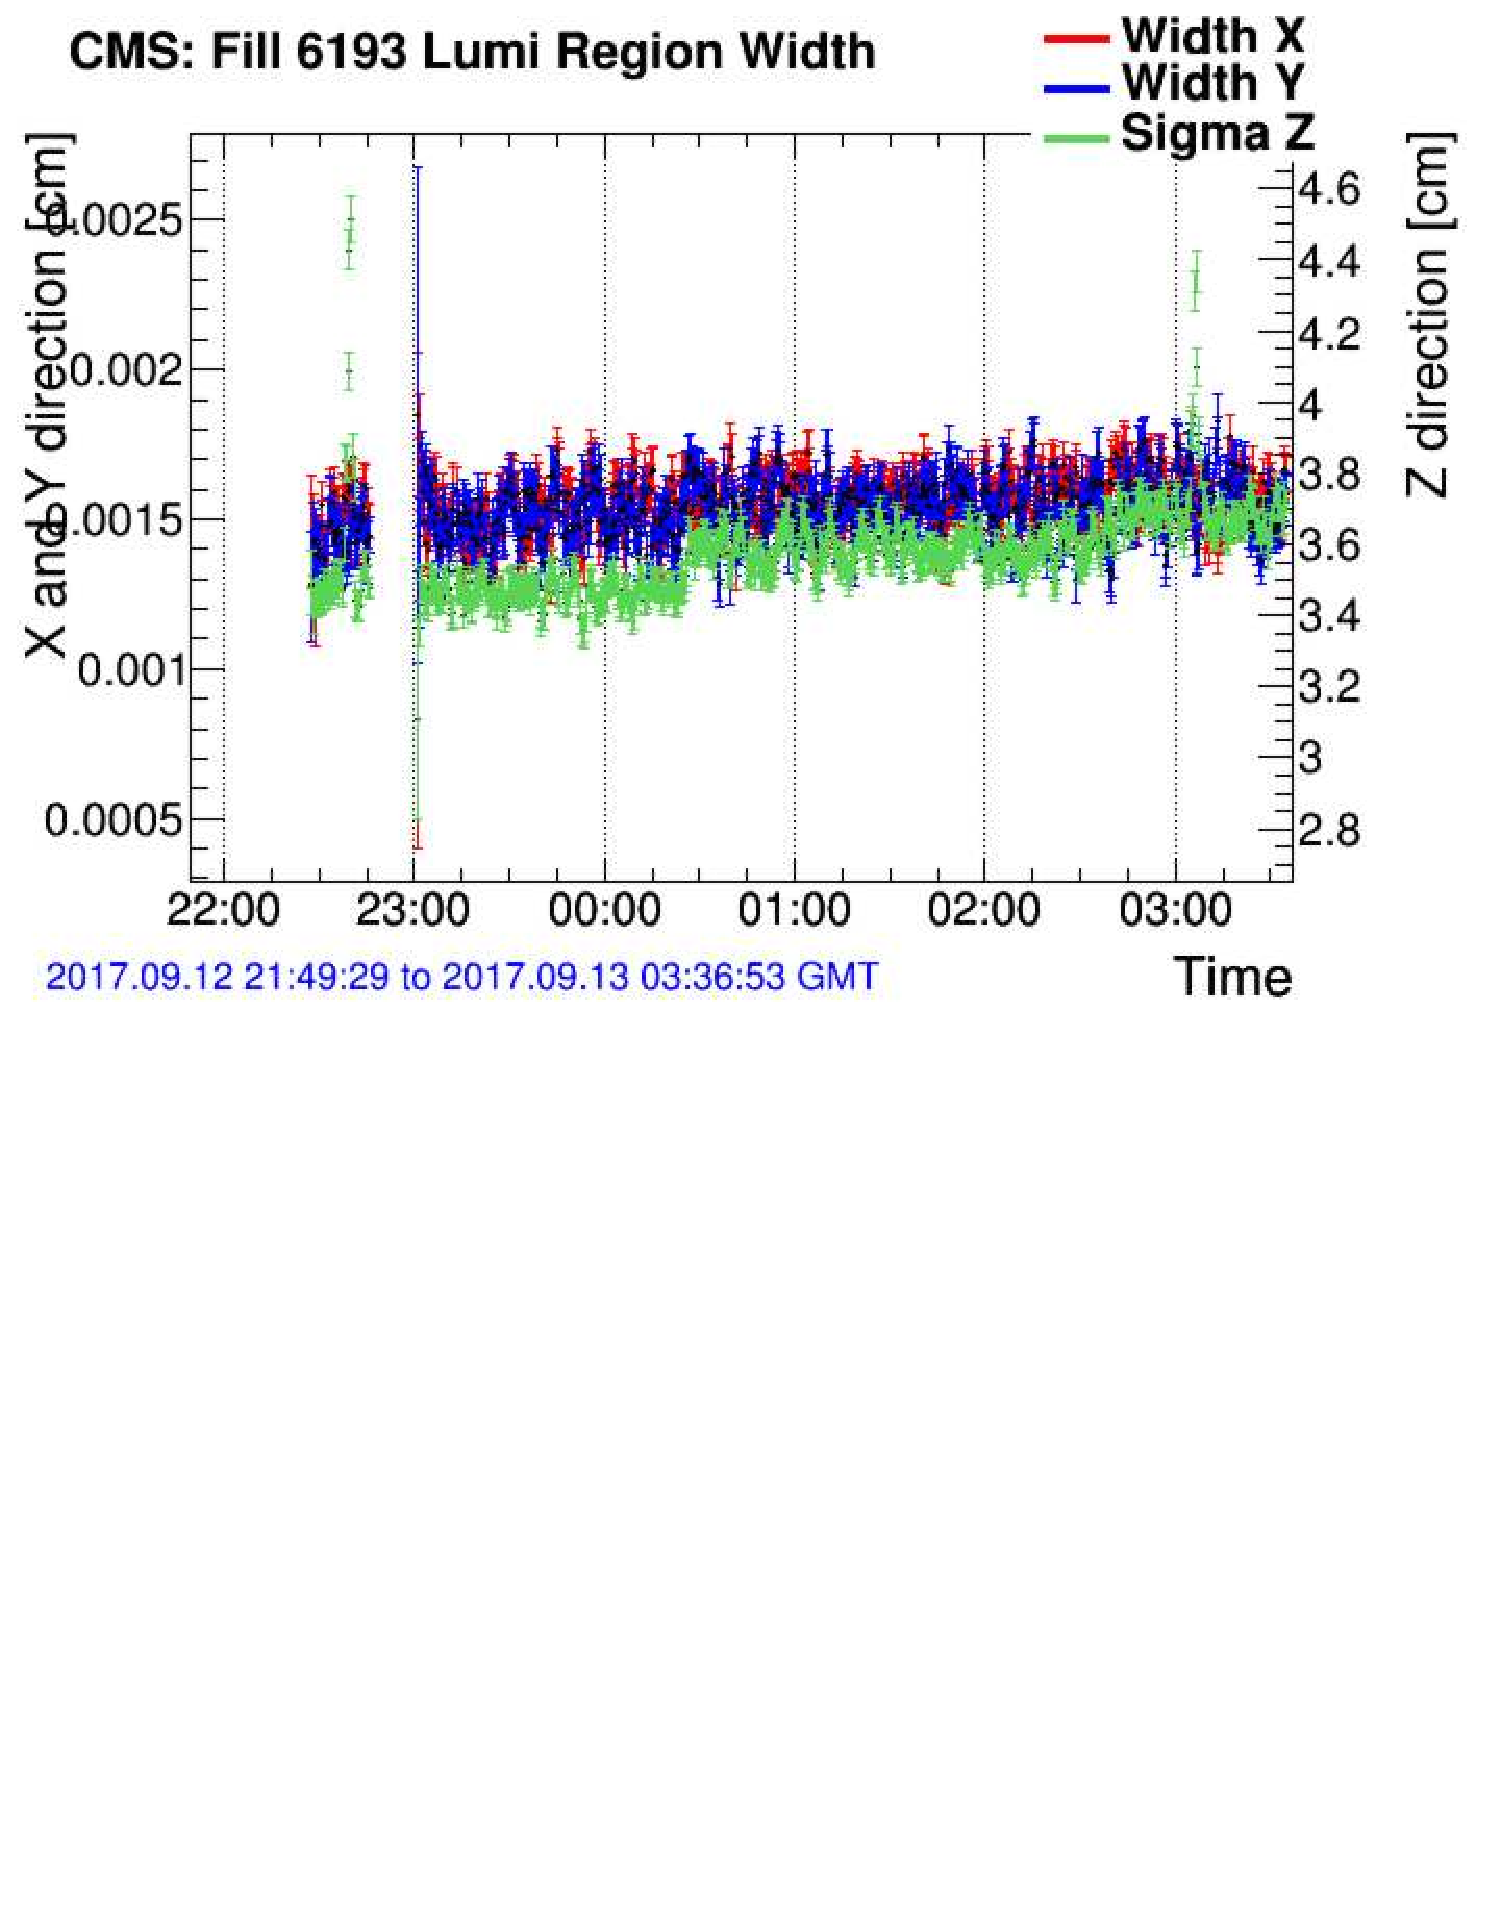
\includegraphics[trim = 0mm 140mm 0mm 0mm, clip, width=0.46\textwidth]{BS_Width_Fill6193_0.pdf}
		\end{figure}\vspace{-4mm}


	\end{block}
	
\end{frame}

\begin{frame}\scriptsize
	\begin{block}{Why $\sigma(x')^{*}=\sigma(x)^{*}/\beta^{*}$ ?}\scriptsize

		\begin{equation}
		    x^{\prime\prime}-k(s)x=0\,,\,\,\,\,\,\,k = \frac{1}{B\cdot\rho} \frac{{\rm d} B_{y}}{{\rm d}x}\,.
		\label{Hillsequation}
		\end{equation}
		\begin{itemize}
			\item Beam equation, harmonic oscillator with magnetic strength $k(s)$
			\item Ansatz: $x(s)=\sqrt{{\color{red}\beta_x(s)}\varepsilon}\cos\left[\phi_x(s)+\phi_0\right]$ and $\phi'=\frac{1}{\beta}$
			\item Its derivative $x(s)'$ is {\color{blue} the beam divergence} and $x(s)'\propto \sqrt{\frac{\varepsilon}{\beta(s)}}\sin(...)$ 
			\item At points $\beta'=0$, see Wilson's book, the thesis of Hubert or mine
			\item Phase space ellipse and area: $\pi\sigma(x)\sigma(x')=\pi\epsilon=constant$ (Liouville theorem)
		\end{itemize}\vspace{2mm}
		The Gaussian shape of $\sigma(x')$ by TOTEM at 13 TeV from CERN preprint:
		\begin{figure}
			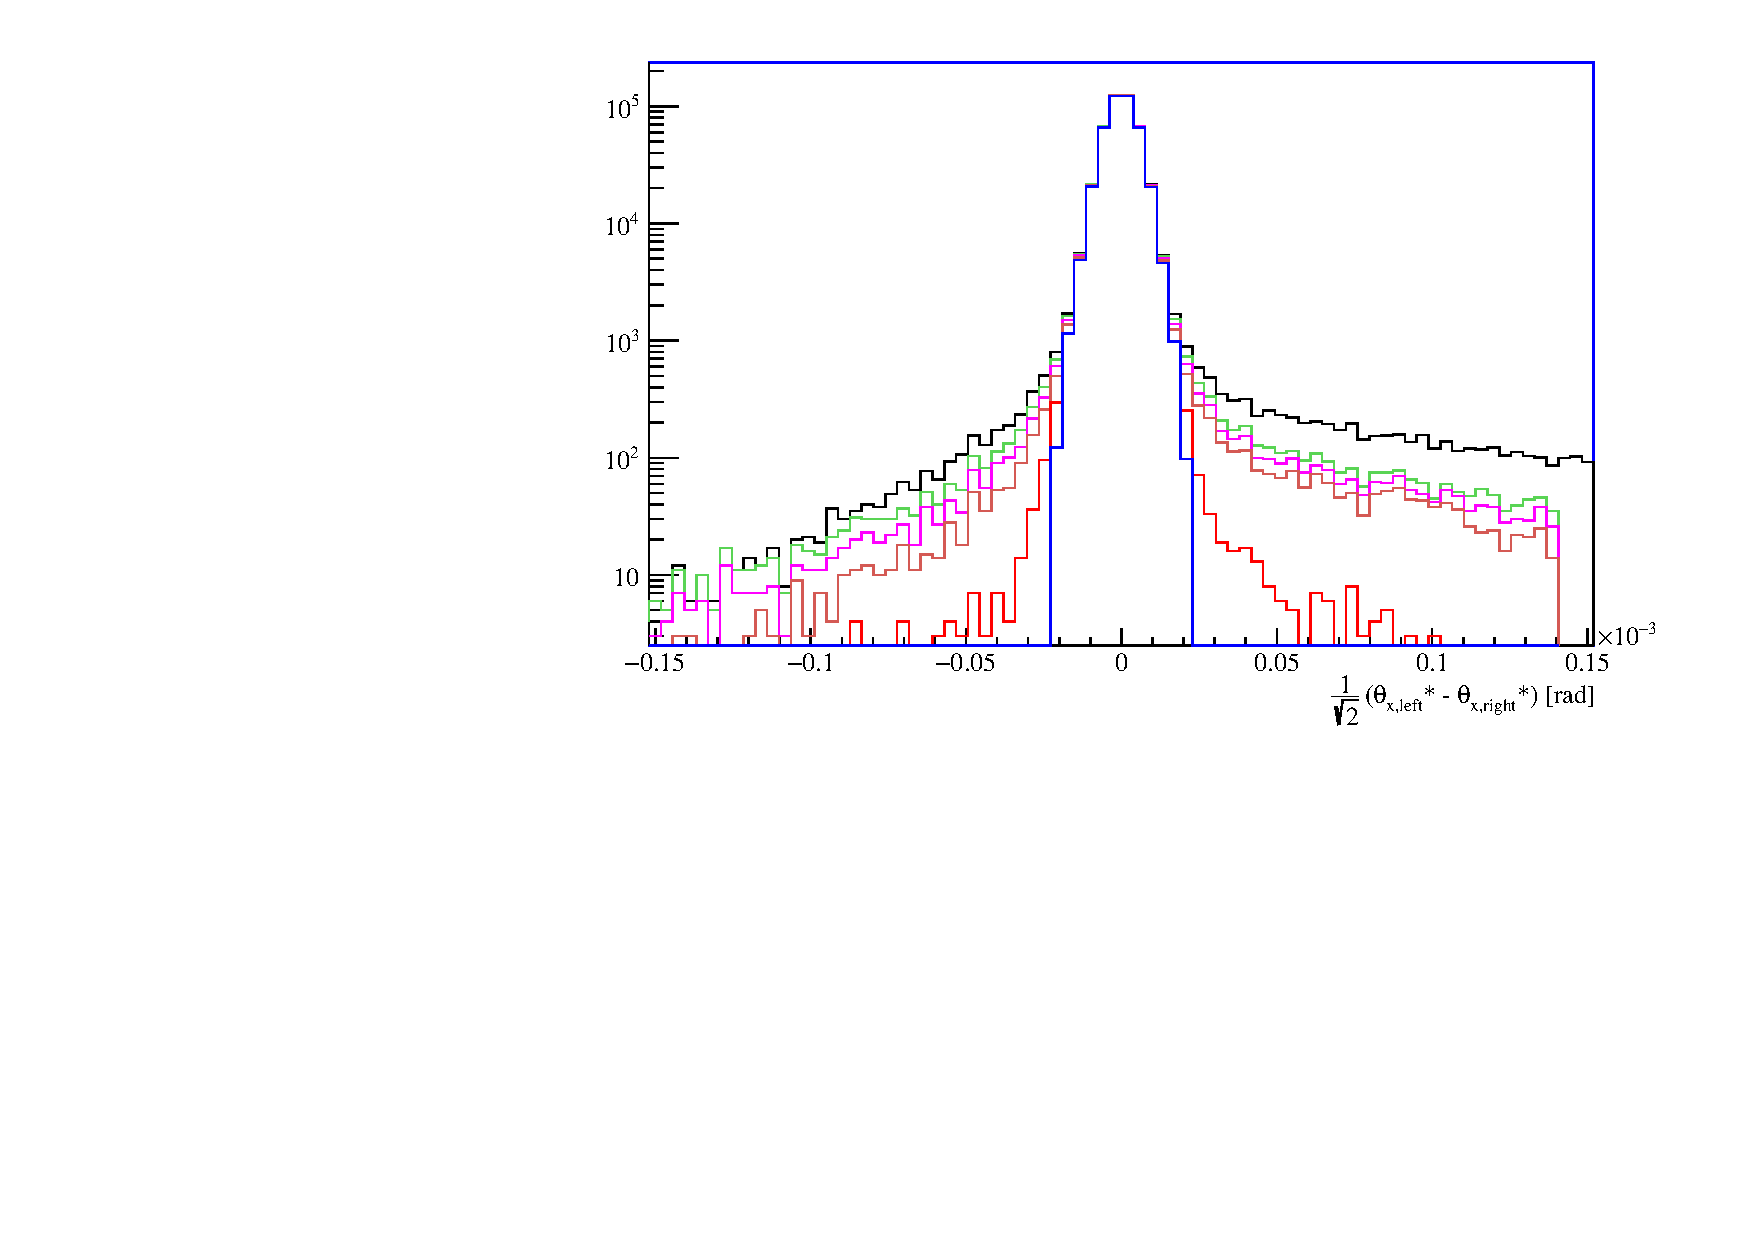
\includegraphics[width=0.46\textwidth]{signal_to_bkg_fill_4496_data_from_cut_definition.pdf}
		\end{figure}\vspace{-4mm}
	\end{block}

	
\end{frame}

\begin{frame}\scriptsize
	\begin{block}{Summary}\scriptsize

		\begin{itemize}
			\item New and reliable method for "neck" position measurement
			\item Applied for available $x$-angles: remains close to 2017 
			\item Rigorous test of alignment / optics assumptions
			\item Beam divergence notes
		\end{itemize}\vspace{10mm}
		{\bf Note}: alignment data with more $x$-angle combination would be useful. Now we have almost only 130~$\mu$rad!
	\end{block}

	
\end{frame}



\end{document}
